% !Mode:: "TeX:UTF-8"

\def\usewhat{pdflatex}                               % 定义编译方式 dvipdfmx 或者 pdflatex,默认为 dvipdfmx
                                                     % 方式编译,如果需要修改,只需改变花括号中的内容即可。
\documentclass[12pt,openany,oneside,ctexartutf8]{book}
                                                     % 本科生毕业论文通常采用单页排版
% !Mode:: "TeX:UTF-8"
%  Authors: 张井   Jing Zhang: prayever@gmail.com     天津大学2010级管理与经济学部信息管理与信息系统专业硕士生
%           余蓝涛 Lantao Yu: lantaoyu1991@gmail.com  天津大学2008级精密仪器与光电子工程学院测控技术与仪器专业本科生

%%%%%%%%%% Package %%%%%%%%%%%%
\usepackage{graphicx}                       % 支持插图处理
% \usepackage[a4paper,text={146.4true mm,239.2 true mm},top= 25.4true mm, bottom= 25.4true mm, left=31.7 true mm,head=6true mm,headsep=6.5true mm,foot=16.5true mm]{geometry}
\usepackage[a4paper,top=25.4mm, bottom=25.4mm, left=31.7mm, right=31.7mm, head=6true mm,headsep=6.5true mm,foot=17.5mm]{geometry}
                                            % 支持版面尺寸设置
\usepackage[squaren]{SIunits}               % 支持国际标准单位

\usepackage{titlesec}                       % 控制标题的宏包
\usepackage{titletoc}                       % 控制目录的宏包
\usepackage{fancyhdr}                       % fancyhdr宏包 支持页眉和页脚的相关定义
\usepackage[UTF8]{ctex}                     % 支持中文显示
\usepackage{CJKpunct}
\usepackage{color}                          % 支持彩色
\usepackage{amsmath}                        % AMSLaTeX宏包 用来排出更加漂亮的公式
\usepackage{amssymb}                        % 数学符号生成命令
\usepackage[below]{placeins}    %允许上一个section的浮动图形出现在下一个section的开始部分,还提供\FloatBarrier命令,使所有未处理的浮动图形立即被处理
\usepackage{multirow}                       % 使用Multirow宏包,使得表格可以合并多个row格
\usepackage{booktabs}                       % 表格,横的粗线;\specialrule{1pt}{0pt}{0pt}
\usepackage{longtable}                      % 支持跨页的表格。
\usepackage{tabularx}                       % 自动设置表格的列宽
\usepackage{subfigure}                      % 支持子图 %centerlast 设置最后一行是否居中
\usepackage[subfigure]{ccaption}            % 支持子图的中文标题
\usepackage[sort&compress,numbers]{natbib}  % 支持引用缩写的宏包
\usepackage{enumitem}                       % 使用enumitem宏包,改变列表项的格式
\usepackage{calc}                           % 长度可以用+ - * / 进行计算
\usepackage{txfonts}                        % 字体宏包
\usepackage{bm}                             % 处理数学公式中的黑斜体的宏包
\usepackage[amsmath,thmmarks,hyperref]{ntheorem}  % 定理类环境宏包,其中 amsmath 选项用来兼容 AMS LaTeX 的宏包
\usepackage{CJKnumb}                        % 提供将阿拉伯数字转换成中文数字的命令
\usepackage{indentfirst}                    % 首行缩进宏包
\usepackage{CJKutf8}                        % 用在UTF8编码环境下,它可以自动调用CJK,同时针对UTF8编码作了设置

% \usepackage{fancybox} 

%\usepackage{hypbmsec}                      % 用来控制书签中标题显示内容
\newcommand{\tabincell}[2]{\begin{tabular}{@{}#1@{}}#2\end{tabular}}
\usepackage{xcolor}
%支持代码环境
\usepackage{listings}
\lstset{numbers=left,
language=[ANSI]{C},
numberstyle=\tiny,
extendedchars=false,
showstringspaces=false,
breakatwhitespace=false,
breaklines=true,
captionpos=b,
keywordstyle=\color{blue!70},
commentstyle=\color{red!50!green!50!blue!50},
frame=shadowbox,
rulesepcolor=\color{red!20!green!20!blue!20}
}
%支持算法环境
\usepackage[boxed,ruled,lined]{algorithm2e}
\usepackage{algorithmic}

\usepackage{array}
\newcommand{\PreserveBackslash}[1]{\let\temp=\\#1\let\\=\temp}
\newcolumntype{C}[1]{>{\PreserveBackslash\centering}p{#1}}
\newcolumntype{R}[1]{>{\PreserveBackslash\raggedleft}p{#1}}
\newcolumntype{L}[1]{>{\PreserveBackslash\raggedright}p{#1}}

% 生成有书签的 pdf 及其生成方式。通常可以在 tjumain.tex 文件的第一行选择 pdflatex 或者是 dvipdfmx 编译手段。如果选择前者,则使用 pdflatex + pdflatex 编译; 如果选择后者,在编译的时候选择 latex + bibtex + latex + latex 编译。出现混淆的时候,系统会报错。
% 如果您的pdf制作中文书签有乱码使用如下命令,就可以解决了
\def\atemp{pdflatex}\ifx\atemp\usewhat
\usepackage{cmap}                           % pdflatex 编译时,可以生成可复制、粘贴的中文 PDF 文档, 缺点是在Windows上显示时效果不大好,字体发虚
\usepackage{hyperref}
\hypersetup{
    unicode,
    pdfborder={0 0 0},
}
\fi
% \usepackage[pdftex,unicode,
%             CJKbookmarks=true,
%             bookmarksnumbered=true,
%             bookmarksopen=true,
%             colorlinks=false,
%             pdfborder={0 0 0},
%             citecolor=blue,
%             linkcolor=red,
%             anchorcolor=green,
%             urlcolor=blue,
%             breaklinks=true
%             ]{hyperref}

                                % 定义本文所使用宏包
\graphicspath{{figures/}}                            % 定义所有的 .eps 文件在 figures 子目录下
\begin{document}                                     % 开始全文
\begin{CJK*}{UTF8}{song}                             % 开始中文字体使用
	% !Mode:: "TeX:UTF-8"
%  Authors: 张井   Jing Zhang: prayever@gmail.com     天津大学2010级管理与经济学部信息管理与信息系统专业硕士生
%           余蓝涛 Lantao Yu: lantaoyu1991@gmail.com  天津大学2008级精密仪器与光电子工程学院测控技术与仪器专业本科生

% 2018/5/23修正
%           李幼萌 Youmeng Li: liyoumeng@tju.edu.cn   天津大学软件学院软件工程系

%%%%%%%%%%%%%%%%% Fonts Definition and Basics %%%%%%%%%%%%%%%%%
\newcommand{\song}{\CJKfamily{song}}    % 宋体
\newcommand{\fs}{\CJKfamily{fs}}        % 仿宋体
\newcommand{\kai}{\CJKfamily{kai}}      % 楷体
\newcommand{\hei}{\CJKfamily{hei}}      % 黑体
\newcommand{\li}{\CJKfamily{li}}        % 隶书
\newcommand{\yihao}{\fontsize{26pt}{26pt}\selectfont}       % 一号, 单倍行距
\newcommand{\xiaoyi}{\fontsize{24pt}{24pt}\selectfont}      % 小一, 单倍行距
\newcommand{\erhao}{\fontsize{22pt}{1.25\baselineskip}\selectfont}       % 二号, 1.25倍行距
\newcommand{\xiaoer}{\fontsize{18pt}{18pt}\selectfont}      % 小二, 单倍行距
\newcommand{\sanhao}{\fontsize{16pt}{16pt}\selectfont}      % 三号, 单倍行距
\newcommand{\xiaosan}{\fontsize{15pt}{15pt}\selectfont}     % 小三, 单倍行距
\newcommand{\sihao}{\fontsize{14pt}{14pt}\selectfont}       % 四号, 单倍行距
\newcommand{\xiaosi}{\fontsize{12pt}{12pt}\selectfont}      % 小四, 单倍行距
\newcommand{\wuhao}{\fontsize{10.5pt}{10.5pt}\selectfont}   % 五号, 单倍行距
\newcommand{\xiaowu}{\fontsize{9pt}{9pt}\selectfont}        % 小五, 单倍行距

\CJKtilde  % 重新定义了波浪符~的意义
\newcommand\prechaptername{第}
\newcommand\postchaptername{章}

\punctstyle{hangmobanjiao}             % 调整中文字符的表示,行内占一个字符宽度,行尾占半个字符宽度

% 调整罗列环境的布局
\setitemize{leftmargin=3em,itemsep=0em,partopsep=0em,parsep=0em,topsep=-0em}
\setenumerate{leftmargin=3em,itemsep=0em,partopsep=0em,parsep=0em,topsep=0em}

% 避免宏包 hyperref 和 arydshln 不兼容带来的目录链接失效的问题。
\def\temp{\relax}
\let\temp\addcontentsline
\gdef\addcontentsline{\phantomsection\temp}

% 自定义项目列表标签及格式 \begin{publist} 列表项 \end{publist}
\newcounter{pubctr} %自定义新计数器
\newenvironment{publist}{%%%%%定义新环境
\begin{list}{[\arabic{pubctr}]} %%标签格式
    {
     \usecounter{pubctr}
     \setlength{\leftmargin}{2.5em}   % 左边界 \leftmargin =\itemindent + \labelwidth + \labelsep
     \setlength{\itemindent}{0em}     % 标号缩进量
     \setlength{\labelsep}{1em}       % 标号和列表项之间的距离,默认0.5em
     \setlength{\rightmargin}{0em}    % 右边界
     \setlength{\topsep}{0ex}         % 列表到上下文的垂直距离
     \setlength{\parsep}{0ex}         % 段落间距
     \setlength{\itemsep}{0ex}        % 标签间距
     \setlength{\listparindent}{0pt}  % 段落缩进量
    }}
{\end{list}}

\makeatletter
\renewcommand\normalsize{
  \@setfontsize\normalsize{12pt}{12pt} % 小四对应 12 pt
  \setlength\abovedisplayskip{4pt}
  \setlength\abovedisplayshortskip{4pt}
  \setlength\belowdisplayskip{\abovedisplayskip}
  \setlength\belowdisplayshortskip{\abovedisplayshortskip}
  \let\@listi\@listI}
\def\defaultfont{\renewcommand{\baselinestretch}{1.63}\normalsize\selectfont} % 设置行距

\renewcommand{\CJKglue}{\hskip -0.1 pt plus 0.08\baselineskip} % 控制字间距,使每行 34 个汉字
\makeatother

%%%%%%%%%%%%% Contents %%%%%%%%%%%%%%%%%
\renewcommand{\contentsname}{目\qquad 录}
\setcounter{tocdepth}{1} % 控制目录深度
\titlecontents{chapter}[2em]{\vspace{.5\baselineskip}\xiaosan\song}
             {\prechaptername\CJKnumber{\thecontentslabel}\postchaptername\qquad}{}
             {\hspace{.5em}\titlerule*[10pt]{$\cdot$}\sihao\contentspage}
\titlecontents{section}[4.2em]{\vspace{.25\baselineskip}\sihao\song}
             {\thecontentslabel\quad}{}
             {\hspace{.5em}\titlerule*[10pt]{$\cdot$}\sihao\contentspage}
% \titlecontents{subsection}[4em]{\vspace{.25\baselineskip}\xiaosi\song}
%              {\thecontentslabel\quad}{}
%              {\hspace{.5em}\titlerule*[10pt]{$\cdot$}\sihao\contentspage}

%%%%%%%%%% Chapter and Section %%%%%%%%%%%%%
\setcounter{secnumdepth}{4}
\setlength{\parindent}{2em}

\renewcommand{\chaptername}{\prechaptername\CJKnumber{\thechapter}\postchaptername}
\titleformat{\chapter}{\centering}{\xiaosan\song}{\chaptername}{} %{2em}
\titlespacing{\chapter}{0pt}{0.1\baselineskip}{0.8\baselineskip}

\titleformat{\section}{\sihao\hei}{\thesection}{1em}{}
\titlespacing{\section}{0pt}{0.15\baselineskip}{0.25\baselineskip}

\titleformat{\subsection}{\sihao\hei}{\thesubsection}{1em}{}
\titlespacing{\subsection}{0pt}{0.1\baselineskip}{0.3\baselineskip}

\titleformat{\subsubsection}{\sihao\hei}{\thesubsubsection}{1em}{}
\titlespacing{\subsubsection}{0pt}{0.05\baselineskip}{0.1\baselineskip}

%%%%%%%%%% Table, Figure and Equation %%%%%%%%%%%%%%%%%
\renewcommand{\tablename}{表}                                     % 插表题头
\renewcommand{\figurename}{图}                                    % 插图题头
\renewcommand{\thefigure}{\arabic{chapter}-\arabic{figure}}       % 使图编号为 7-1 的格式 %\protect{~}
\renewcommand{\thesubfigure}{\alph{subfigure})}                   % 使子图编号为 a) 的格式
\renewcommand{\thesubtable}{(\alph{subtable})}                    % 使子表编号为 (a) 的格式
\renewcommand{\thetable}{\arabic{chapter}-\arabic{table}}         % 使表编号为 7-1 的格式
\renewcommand{\theequation}{\arabic{chapter}-\arabic{equation}}   % 使公式编号为 7-1 的格式

%%%%%% 定制浮动图形和表格标题样式 %%%%%%
\makeatletter
\long\def\@makecaption#1#2{
   \vskip\abovecaptionskip
   \sbox\@tempboxa{\centering\wuhao\song{#1\qquad #2} }
   \ifdim \wd\@tempboxa >\hsize
     \centering\wuhao\song{#1\qquad #2} \par
   \else
     \global \@minipagefalse
     \hb@xt@\hsize{\hfil\box\@tempboxa\hfil}
   \fi
   \vskip\belowcaptionskip}
\makeatother
\captiondelim{~~~~} %用来控制longtable表头分隔符

%%%%%%%%%% Theorem Environment %%%%%%%%%%%%%%%%%
\theoremstyle{plain}
\theorembodyfont{\song\rmfamily}
\theoremheaderfont{\hei\rmfamily}
\newtheorem{theorem}{定理~}[chapter]
\newtheorem{lemma}{引理~}[chapter]
\newtheorem{axiom}{公理~}[chapter]
\newtheorem{proposition}{命题~}[chapter]
\newtheorem{prop}{性质~}[chapter]
\newtheorem{corollary}{推论~}[chapter]
\newtheorem{definition}{定义~}[chapter]
\newtheorem{conjecture}{猜想~}[chapter]
\newtheorem{example}{例~}[chapter]
\newtheorem{remark}{注~}[chapter]
%\newtheorem{algorithm}{算法~}[chapter]
\newenvironment{proof}{\noindent{\hei 证明:}}{\hfill $ \square $ \vskip 4mm}
\theoremsymbol{$\square$}

%%%%%%%%%% Page: number, header and footer  %%%%%%%%%%%%%%%%%

%\frontmatter 或 \pagenumbering{roman}
%\mainmatter 或 \pagenumbering{arabic}
\makeatletter
\renewcommand\frontmatter{\clearpage
  \@mainmatterfalse
  }
\makeatother

%%%%%%%%%%%% References %%%%%%%%%%%%%%%%%
\renewcommand{\bibname}{参考文献}
% 重定义参考文献样式,来自thu
\makeatletter
\renewenvironment{thebibliography}[1]{
    \titleformat{\chapter}{\raggedright\sihao\hei}{\chaptername}{2em}{}
   \chapter*{\bibname}
   \wuhao
   \list{\@biblabel{\@arabic\c@enumiv}}
        {\renewcommand{\makelabel}[1]{##1\hfill}
         \settowidth\labelwidth{0 cm}
         \setlength{\labelsep}{0pt}
         \setlength{\itemindent}{0pt}
         \setlength{\leftmargin}{\labelwidth+\labelsep}
         \addtolength{\itemsep}{-0.7em}
         \usecounter{enumiv}
         \let\p@enumiv\@empty
         \renewcommand\theenumiv{\@arabic\c@enumiv}}
    \sloppy\frenchspacing
    \clubpenalty4000
    \@clubpenalty \clubpenalty
    \widowpenalty4000
    \interlinepenalty4000
    \sfcode`\.\@m}
   {\def\@noitemerr
     {\@latex@warning{Empty `thebibliography' environment}}
    \endlist\frenchspacing}
\makeatother

\addtolength{\bibsep}{-0.5em}     % 缩小参考文献间的垂直间距
\setlength{\bibhang}{2em}         % 每个条目自第二行起缩进的距离

% 参考文献引用作为上标出现
%\newcommand{\citeup}[1]{\textsuperscript{\cite{#1}}}
\makeatletter
    \def\@cite#1#2{\textsuperscript{[{#1\if@tempswa , #2\fi}]}}
\makeatother
%% 引用格式
\bibpunct{[}{]}{,}{s}{}{,}

%%%%%%%%%%%% Cover %%%%%%%%%%%%%%%%%
% 封面、摘要、版权、致谢格式定义
\makeatletter
\def\ctitle#1{\def\@ctitle{#1}}\def\@ctitle{}
\def\cdegree#1{\def\@cdegree{#1}}\def\@cdegree{}
\def\caffil#1{\def\@caffil{#1}}\def\@caffil{}
\def\csubject#1{\def\@csubject{#1}}\def\@csubject{}
\def\cgrade#1{\def\@cgrade{#1}}\def\@cgrade{}
\def\cauthor#1{\def\@cauthor{#1}}\def\@cauthor{}
\def\cnumber#1{\def\@cnumber{#1}}\def\@cnumber{}
\def\cstuid#1{\def\@cstuid{#1}}\def\@cstuid{}
\def\cdate#1{\def\@cdate{#1}}\def\@cdate{}
\long\def\cabstract#1{\long\def\@cabstract{#1}}\long\def\@cabstract{}
\long\def\eabstract#1{\long\def\@eabstract{#1}}\long\def\@eabstract{}
\def\ckeywords#1{\def\@ckeywords{#1}}\def\@ckeywords{}
\def\ekeywords#1{\def\@ekeywords{#1}}\def\@ekeywords{}
\def\cheading#1{\def\@cheading{#1}}\def\@cheading{}
\def\ccovertitle#1{\def\@ccovertitle{#1}}\def\@ccovertitle{}

\pagestyle{fancy}
  \fancyhf{}
  \fancyhead[C]{\song\wuhao \@cheading}  % 页眉显示天津大学 20XX 届本科生毕业论文
  \fancyfoot[C]{\song\xiaowu ~\thepage~}
\newlength{\@title@width}

% 定义封面
\def\makecover{
%\cleardoublepage%
   \phantomsection
    \pdfbookmark[-1]{\@ctitle}{ctitle}

    \begin{titlepage}
      \vspace*{10pt}
      \begin{center}

      \begin{figure}[h]
      \centering
      
\includegraphics[width=0.4\textwidth]{figures/tju}
      \end{figure}
      \vspace*{15pt}
      \hei\erhao{\textbf{\@ccovertitle}} \\
      \hei\erhao{\textbf{\@ctitle}}
      \vspace*{55pt}

      \begin{figure}[h]
      \centering
      
\includegraphics[width=0.3\textwidth]{figures/Tjulogo}
      \end{figure}

      \vspace*{60pt}
      \renewcommand\arraystretch{1.5}
      \setlength{\@title@width}{12cm}
      {
        \sanhao\song{
          \begin{tabular}{lc}
            \textbf{学\qquad 院}  &  \underline{\makebox[\@title@width][c]{\textbf{\@caffil}}} \\
            \textbf{专\qquad 业}  &  \underline{\makebox[\@title@width][c]{\textbf{\@csubject}}} \\
            \textbf{年\qquad 级}  &  \underline{\makebox[\@title@width][c]{\textbf{\@cgrade}}}\\
            \textbf{姓\qquad 名}  &  \underline{\makebox[\@title@width][c]{\textbf{\@cauthor}}}\\
            \textbf{学\qquad 号}  &  \underline{\makebox[\@title@width][c]{\textbf{\normalsize\@cstuid}}}\\
          \end{tabular}
        }
    }
    \vspace*{40pt}

    \song\sanhao{\textbf{\@cdate}}
    \end{center}
    \end{titlepage}
}

                             % 完成对论文各个部分格式的设置
	% !Mode:: "TeX:UTF-8"


%%%%%%%%%%%%%%%%%%%%%%%%%%%%%%%%%%%%%%%%%%%%%%%%%%%%%%%%%%%%%%%
%%  可通过对 setup/format.tex中                               %%
%%  第243行 \setlength{\@title@width}{5cm}中 5cm 这个参数来   %%
%%  控制封面中下划线的长度。                                   %%
%%%%%%%%%%%%%%%%%%%%%%%%%%%%%%%%%%%%%%%%%%%%%%%%%%%%%%%%%%%%%%

\cheading{天津大学软件学院~\the\year~年《软件工程综合实践》实践报告}      % 正文页眉
\ccovertitle{《软件工程综合实践》实践报告}                       % 封面标题

%%%%%%%%%%%%%%%%%%%%%%%%%%%%%%%%%%%%%%%%%%%%%%%%%%%%%%%%%%%%%
%%%%%%%%%% 以下为论文的基本信息,需要由作者进行修改 %%%%%%%%%%%%
%%%%%%%%%%%%%%%%%%%%%%%%%%%%%%%%%%%%%%%%%%%%%%%%%%%%%%%%%%%%%
\ctitle{饿了么~外卖平台}    % 封面用论文标题,自己可手动断行
\caffil{智能与计算学部}       % 学院名称
\csubject{软件工程}     % 专业名称
\cgrade{21级}           % 年级
\cauthor{易东廷 \newline 张中天 \newline 张梅梅 \newline 杜伟乐}          % 学生姓名
\cstuid{3021244187~3021210045~3021244259~6321012105}     % 学号

\cdate{\the\year~年~\the\month~月~\the\day~日}  % 论文完成日期,不需要修改,自动生成

	\frontmatter                                     % 以下是论文导言部分,包括论文的封面,中英文摘要和中文目录
	\fancypagestyle{plain}{							 % 正文前均无页眉
		\fancyhf{}
		\renewcommand{\headrulewidth}{0 pt}
		\fancyfoot[C]{\song\xiaowu~\thepage~}
	}

	\makecover 			% 封面

	% !Mode:: "TeX:UTF-8"

% 目录
\defaultfont
\clearpage{
    \pagestyle{empty}
    \cleardoublepage
    \setcounter{page}{1}                                 % 单独从 1 开始编页码
    \pagenumbering{arabic}
    \titleformat{\chapter}{\centering\sanhao\hei}{\chaptername}{2em}{} % 设置目录两字的格式
    \pdfbookmark[0]{目~~录}{mulu}
    \tableofcontents                                     % 中文目录
    \thispagestyle{plain}
} % 目录

	\mainmatter\defaultfont\sloppy\raggedbottom
	\makeatletter
	\fancypagestyle{plain}{                              % 设置正文眉页脚风格
		\fancyhf{}
		\fancyhead[C]{\song\wuhao \@cheading}            % 页眉格式
		\fancyfoot[C]{\song\xiaowu ~\thepage~}           % 页脚格式
		\renewcommand{\headrulewidth}{0.5pt}
		\renewcommand{\footrulewidth}{0pt}
	}
	\makeatother
	\setcounter{page}{1}                                 % 单独从 1 开始编页码
	\titleformat{\chapter}{\centering\xiaosan\hei}{\chaptername}{2em}{} % 恢复chapter标题格式要求

	%%%%%% 这里是正文,每个文件对应正文中的一章 %%%%%%
	\chapter{团员分工}
\section{Spring Cloud 注册中心}
\begin{itemize}
    \item{项目负责团员}:张梅梅
    \item {项目描述}:本项目主要负责搭建并配置 Eureka Server 注册中心,实现管理服务的注册和发现,确保服务之间的通信顺畅。另外,本项目也需要集成服务路由和负载均衡功能,提高系统的稳定性和性能。
\end{itemize}

\section{Spring Cloud 微服务网关}
\begin{itemize}
    \item{项目负责团员}:张梅梅
    \item {项目描述}:本项目主要负责配置并管理 Spring Cloud Gateway 等网关组件,设置路由规则,并实现请求转发和过滤功能。
\end{itemize}

\section{Spring Cloud 集中配置管理中心}
\begin{itemize}
    \item{项目负责团员}:张中天
    \item {项目描述}:本项目主要负责搭建 Spring Cloud Config Server,用于集中式管理配置信息。此外,需要负责配置Git或其他版本控制系统,用于存储和管理配置文件,最后集成配置中心到项目中,并实现动态配置刷新功能。
\end{itemize}

\section{Spring Cloud 新增微服务架构}
\subsection{积分系统}
\begin{itemize}
    \item{项目负责团员}:张中天
    \item {项目描述}:本项目主要负责设计积分系统的数据库结构,包括用户积分表、积分规则表等。此外,本项目需开发积分交易接口,包括积分查询、积分兑换等功能,并且实现积分计算逻辑,根据订单金额、活动规则等计算用户应得积分。
\end{itemize}

\subsection{虚拟钱包系统}
\begin{itemize}
    \item{项目负责团员}:张中天
    \item {项目描述}:本项目主要负责设计钱包系统的数据库结构,包括用户钱包表、交易记录表等,并实现虚拟钱包功能,包括余额查询、充值、提现等。本项目的主要目的是为了实现外卖平台的支付流程,以让外卖平台的操作更方便且具人性化。
\end{itemize}

\subsection{身份校验}
\begin{itemize}
    \item{项目负责团员}:易东廷
    \item {项目描述}:本项目主要负责设计用户身份验证流程,包括注册、登录、认证等环节。本项目具体需要开发用户注册和登录接口,实现用户身份信息的验证和存储,并集成第三方身份验证服务,增强登录状态的管理和用户权限的控制。
\end{itemize}

\section{Spring Cloud 基础微服务架构}
\subsection{用户服务}
\begin{itemize}
    \item{项目负责团员}:易东廷
    \item {项目描述}:本项目主要负责开发用户微服务的功能,包括开发用户注册、登录和个人信息管理功能,并实现用户权限管理功能,包括用户角色、权限分配等。
\end{itemize}

\subsection{地址服务}
\begin{itemize}
    \item{项目负责团员}:易东廷
    \item {项目描述}:本项目主要负责开发用户收货地址微服务的管理功能,包括添加、修改、删除地址信息。
\end{itemize}

\subsection{商家服务}
\begin{itemize}
    \item{项目负责团员}:杜伟乐
    \item {项目描述}:本项目主要负责开发商家微服务的管理功能,包括商家名称、商家信息、商家地址等。本项目主要用于用户在使用平台时可以游览所支持的商家,并选择指定商家进行点餐。
\end{itemize}

\subsection{食品服务}
\begin{itemize}
    \item{项目负责团员}:杜伟乐
    \item {项目描述}:本项目主要负责开发外卖食品微服务的管理功能,实现菜单查询接口,用于用户浏览和点餐。
\end{itemize}

\subsection{购物车服务}
\begin{itemize}
    \item{项目负责团员}:于鑫慧
    \item {项目描述}:本项目主要负责开发购物车服务的管理功能,包括商品添加、删除、数量修改等。此外,本项目也需要实现购物车与订单的关联,确保购物车中的商品可以正确结算。
\end{itemize}

\subsection{点餐服务}
\begin{itemize}
    \item{项目负责团员}:于鑫慧
    \item {项目描述}:本项目主要负责开发点餐微服务的核心功能,包括菜品浏览、加入购物车、下单等。此外,本项目也需要实现订单管理功能,包括订单查询、订单状态更新等。
\end{itemize}

\section{项目云部署}
\begin{itemize}
    \item{项目负责团员}:张中天
    \item{项目描述}:本项目主要负责选择合适的云服务提供商,并将项目部署到云服务器上。另外,本项目需要配置云服务器环境,包括虚拟机、数据库、存储等,并实现持续集成和持续部署流程,确保项目的稳定性和安全性。    
\end{itemize}

\section{项目文档}
\begin{itemize}
    \item{项目负责团员}:杜伟乐
    \item{项目描述}:本项目主要负责书写本项目文档的内容,其中内容包括了本软件的团员分工和需求分析。
\end{itemize}

\section{项目测试}
\begin{itemize}
    \item{项目负责团员}:张梅梅、于鑫慧
    \item{项目描述}:本项目主要负责对项目进行单元测试,验证每个模块的功能和逻辑是否符合预期。此外,本项目也需要进行集成测试,测试不同模块之间的交互和整体功能,以及进行系统测试,模拟真实场景,验证系统的性能和稳定性。
\end{itemize}

\section{项目演示}
\begin{itemize}
    \item{项目负责团员}:张梅梅
    \item{项目描述}:本项目主要负责演示项目的核心功能和特点,包括展示外卖平台的用户界面和具体点餐操作流程。
\end{itemize}






 %任务分工
	\chapter{项目需求}

\section{系统背景}
在过去的几十年中,餐饮行业一直是人们生活中重要的组成部分。然而,随着城市化和工作压力的增加,传统的进餐方式面临着许多挑战。人们的时间日益宝贵,越来越多的人选择在家或办公室点外卖,以节省时间和精力。这为外卖平台的崛起提供了机会。随着智能手机的普及,移动互联网的兴起以及在线支付的便捷性,外卖平台逐渐演变成一个综合性的餐饮服务平台,为用户提供了更加便利、多样化的选择。

“饿了么”外卖平台为用户和餐厅提供了一个互相连接的桥梁,具有以下核心功能:
\begin{itemize}
    \item{\textbf{用户点餐}}:用户通过“饿了么”移动应用程序或网站浏览附近的餐厅和菜单,并可以根据自己的口味和需求下订单。
    \item{\textbf{多样选择}}:平台上的餐厅涵盖了各种菜系,从传统美食到国际化的料理,满足了用户不同的口味偏好。
    \item{\textbf{配送服务}}:“饿了么”为用户提供送餐服务,用户可以实时跟踪订单状态,知道餐食的准确送达时间。
    \item{\textbf{在线支付}}:用户可以通过平台进行在线支付,不需要现金交易,实现O2O(Online~to~Offline)外卖模式
    \item{\textbf{评价和评论}}:用户可以对餐厅和菜品进行评价和评论,帮助其他用户做出更好的选择。
    \item{\textbf{营销活动}}:平台定期推出各种促销活动和优惠券,吸引用户下单并提升用户粘性。
\end{itemize}

\section{系统架构}
\subsection{饿了么外卖平台系统架构描述}
本软件采用前后端分离的开发方式,为移动端开发一个外卖平台软件。
\begin{itemize}
    \item {数据库}:
    \item {后端}:
    \item {前端}:首先采用~HTML5、~CSS3~和~JavaScript~语言的相关技术开发外卖平台的静态页面。其次采用~Vue3~架构构造一个与后端交互的前端页面。
\end{itemize}
\subsection{饿了么外卖平台系统架构图}

\section{业务架构}
\subsection{用户点餐业务流程描述}
首先,用户在首页选择了相应的商家分类,便会跳转至对应的商家列表页面。在商家页表页面里,用户选择相应的商家并跳转至对应的商家信息页面。在商家信息页面里,用户可以选择往购物车里添加或删除菜品。当用户选择完毕,并会跳转至确认订单页面。

在确认订单页面中,用户可以选择送货地址以及检查自己的订单是否正确,确认无误后就会跳转至在线支付页面。在此页面中,用户可以选择不同的第三方支付方式并确认支付。点餐业务到此结束。
\subsection{用户点餐业务流程图}
本软件的用户点餐流程图如图~\ref{fig:process}~所示。
\begin{figure}[htbp]
    \centering
    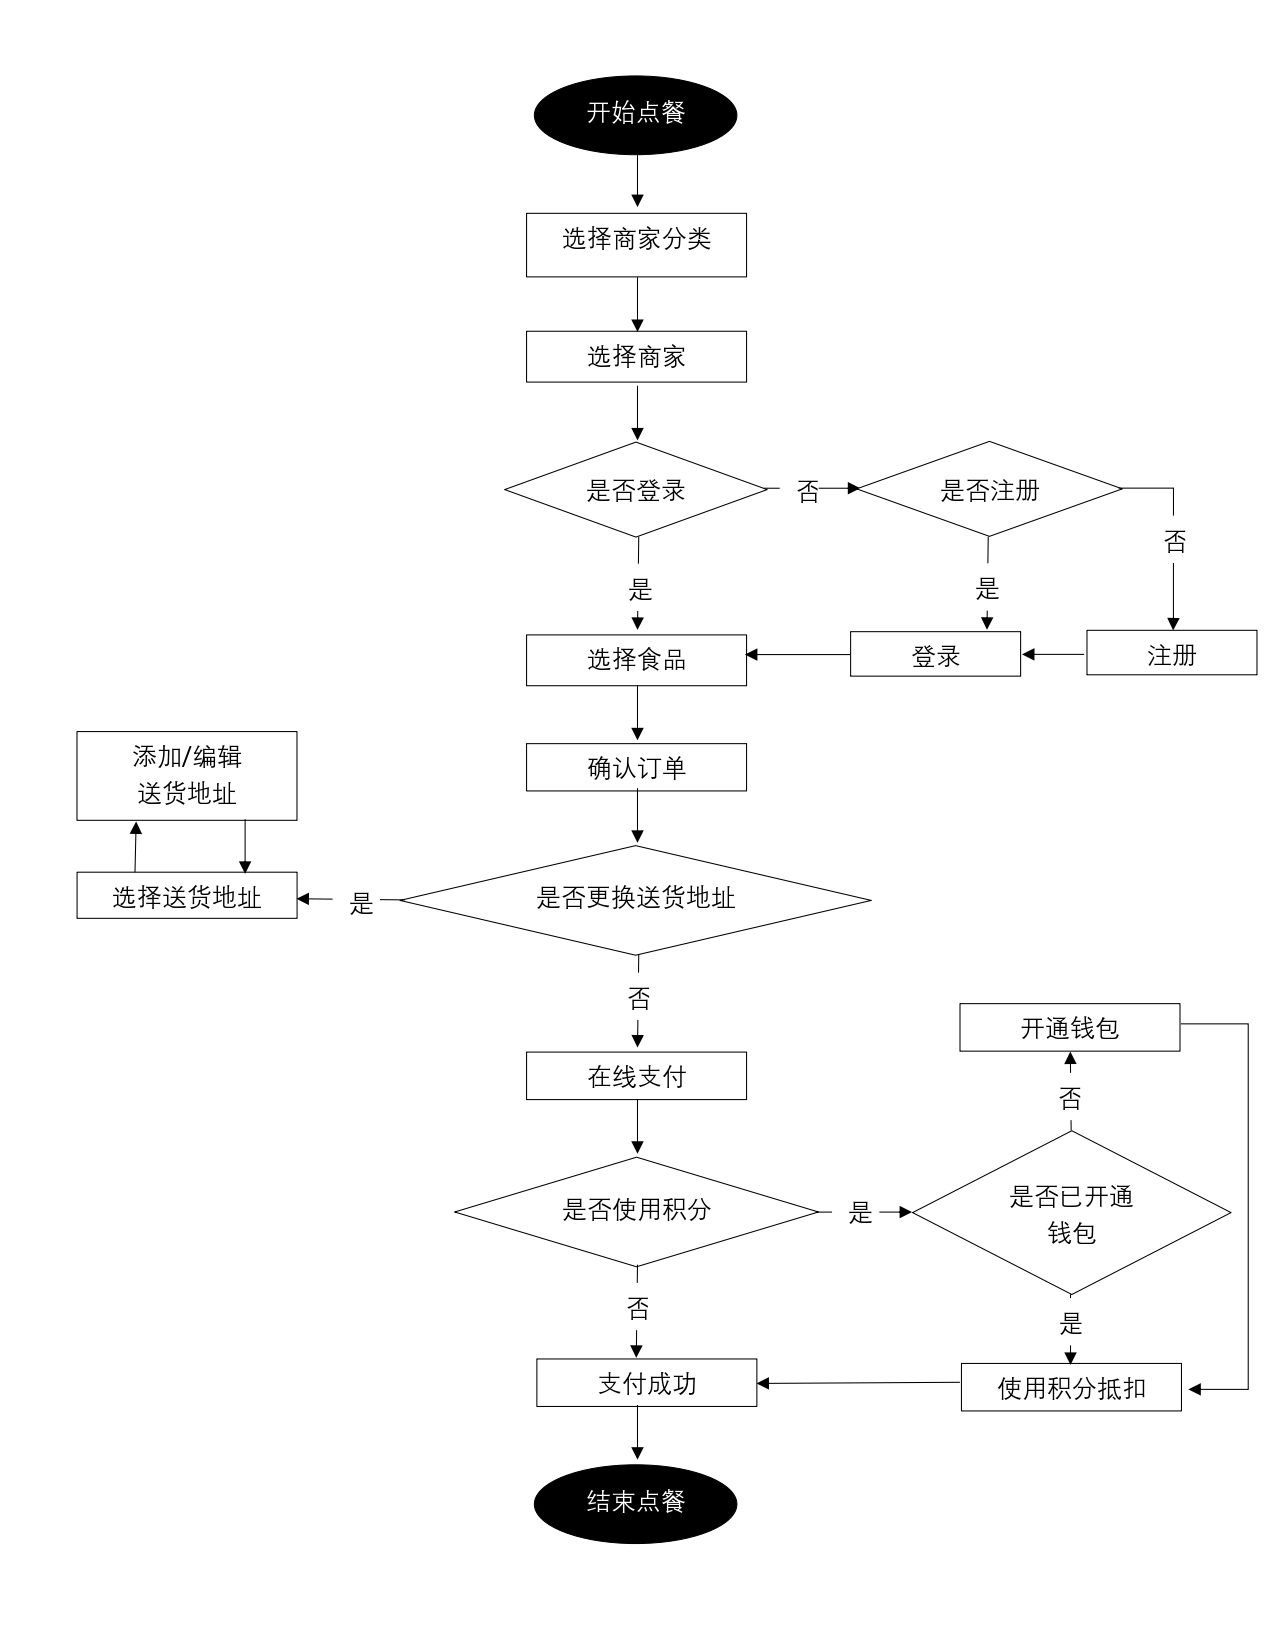
\includegraphics[width=0.8\textwidth]{processmap}
    \caption{饿了么外卖平台用户点餐业务流程图}\label{fig:process}
    \vspace{\baselineskip}
    \end{figure}

\section{用户需求}
本软件由三个用户组成,分别为用户、商家和管理员。用户角色由表~\ref{tab:table1}~所示。
\begin{table}[htbp]
\caption{饿了么外卖平台不同用户的功能描述}\label{tab:table1}
\vspace{0.5em}\wuhao
\begin{tabularx}{\textwidth}{llX}
\toprule[1.5pt]
序号 & 用户 & 功能描述 \\ 
\midrule[1pt]
1 & 用户 & 
\begin{itemize}
    \item{\textbf{游览菜品}}:消费者可以在首页浏览附近的餐厅列表。他们可以按照菜系、评分、特别优惠等条件筛选餐厅,了解每家餐厅的菜单和菜品详情。
    \item{\textbf{选择菜品}}:消费者可以根据菜品的图片、描述以及价格做出最合适的选择。
    \item{\textbf{在线支付}}:消费者将所选的菜品添加到购物车,确认订单后选择第三方的支付方式进行支付,完成订单。
    \item {\textbf{管理地址信息}}:消费者可以自行添加、删除和查看收获地址的信息。
    \item {\textbf{管理订单信息}}:消费者可以在历史订单页面查看已生成的订单状态,其中包含已选购的商家和菜品明细。
    \item {\textbf{登陆注册}}:消费者可以通过手机号注册一个饿了么外卖平台的账号。
\end{itemize}
\\
2 & 商家 & 
\begin{itemize}
    \item{\textbf{注册和上架}}:商家需要先在平台上注册自己的餐厅。一旦注册成功,他们可以填写餐厅的基本信息、菜单、菜品描述和价格等。
    \item{\textbf{菜单管理}}:商家可以通过平台管理菜单,包括添加新菜品、修改菜品信息、调整价格等。
    \item{\textbf{接受订单}}:商家在平台上收到订单通知后,可以查看订单详情,包括所点菜品、数量、送达地址以及支付信息。
    \item {\textbf{准备食物}}:商家接受订单后,就可以开始准备食物。
\end{itemize}
\\
3 & 管理员 & 
\begin{itemize}
    \item{\textbf{平台监督和管理}}:管理员负责监督外卖平台的整体运营情况。他们使用管理后台工具,监控平台的性能、稳定性和安全性,确保用户能够顺利访问平台。
    \item{\textbf{监控订单和投诉}}:管理员跟踪订单处理流程,确保订单按时送达。
    \item{\textbf{技术支持和升级}}:管理员负责监督技术团队,确保平台的技术架构和功能持续适应市场需求,并在必要时进行系统更新。
    \item {\textbf{风险管理和安全性}}:管理员制定隐私政策、安全措施,确保用户的个人信息和支付数据得到妥善保护。
\end{itemize}
\\
\bottomrule[1.5pt]
\end{tabularx}
\vspace{\baselineskip}
\end{table}

\section{功能性需求}
\subsection{首页}
首页是本软件的主要页面。此页面展示了用户当前的收货地址、商家搜索栏、菜品分类、推荐商家列表以及其他优惠部分。首页的底部有一个菜单,显示外卖平台的【首页】、【发现】、【订单】以及【我的】按钮。用户可以点击相应的按钮跳转至对应的页面进行操作。
\subsubsection{界面设计}
本软件的首页界面设计如图~\ref{fig:index}~所示。
\begin{figure}[htbp]
\centering
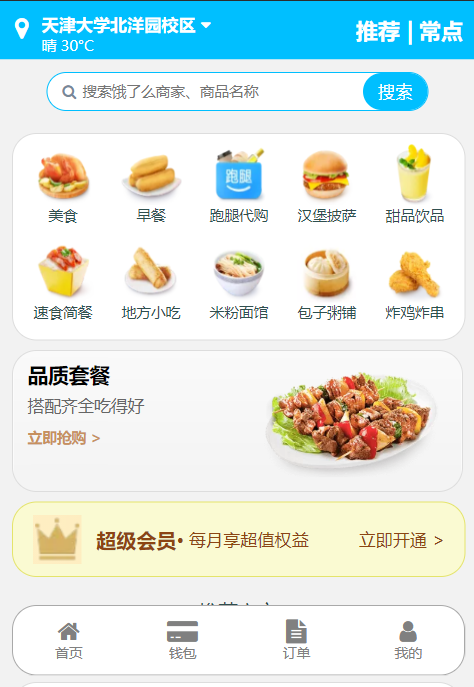
\includegraphics[width=0.4\textwidth]{index}
\caption{首页界面设计}\label{fig:index}
\vspace{\baselineskip}
\end{figure}
\subsubsection{功能按钮}
本软件首页功能按钮如表~\ref{tab:table2}~所示。
\begin{table}[htbp]
    \caption{饿了么外卖平台首页功能按钮}\label{tab:table2}
    \vspace{0.5em}\wuhao
    \begin{tabularx}{\textwidth}{lllX}
    \toprule[1.5pt]
    序号 & 按钮名称 & 功能 & 功能规则 \\ 
    \midrule[1pt]
    1 & 当前送货地址 & 用户选择送货地址 & 点击跳转至地址管理页面。 \\
    2 & 搜索框 & 用户搜索商家名称 & 输入商家名称可根据商家名称查找商家。 \\
    3 & 商家分类 & 用户选择商家分类 & 点击跳转指定商家分类。 \\
    4 & 首页 & 刷新页面 & 点击跳转至首页。 \\
    5 & 订单 & 进入历史订单 & 点击跳转至历史订单页面。 \\
    6 & 我的 & 进入用户信息 & 点击跳转至用户信息页面。 \\
\bottomrule[1.5pt]
\end{tabularx}
\vspace{\baselineskip}
\end{table}

\subsection{商家列表}
当用户在首页点击指定的商家分类后,会跳转至指定分类的商家列表页面。此页面展示了一系列商家,其中包括他们的商家图片、商家名称、商家的起送费、配送费和菜品。
\subsubsection{界面设计}
本软件的商家列表界面设计如图~\ref{fig:businessList}~所示。
\begin{figure}[htbp]
\centering
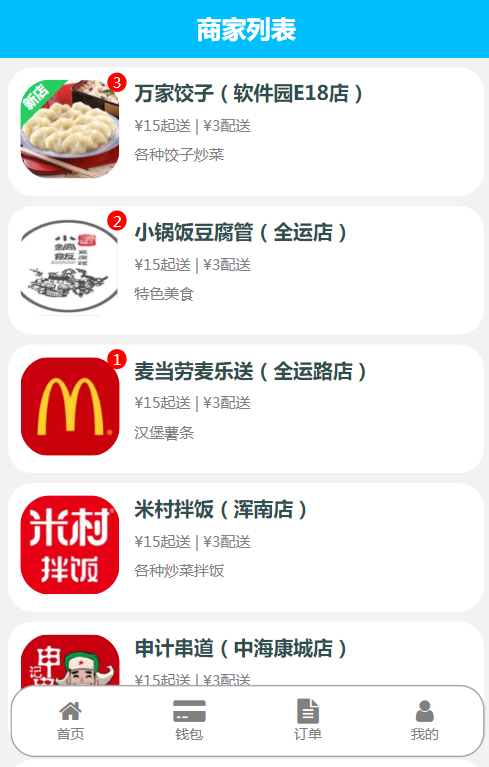
\includegraphics[width=0.4\textwidth]{businessList}
\caption{商家列表界面设计}\label{fig:businessList}
\vspace{\baselineskip}
\end{figure}
\subsubsection{功能按钮}
本软件商家列表功能按钮如表~\ref{tab:table3}~所示。
\begin{table}[htbp]
    \caption{饿了么外卖平台商家列表功能按钮}\label{tab:table3}
    \vspace{0.5em}\wuhao
    \begin{tabularx}{\textwidth}{lllX}
    \toprule[1.5pt]
    序号 & 按钮名称 & 功能 & 功能规则 \\ 
    \midrule[1pt]
    1 & 商家信息 & 用户选择指定商家 & 点击跳转至指定商家信息页面。 \\
    2 & 首页 & 刷新页面 & 点击跳转至首页。 \\
    3 & 订单 & 进入历史订单 & 点击跳转至历史订单页面。 \\
    4 & 我的 & 进入用户信息 & 点击跳转至用户信息页面。 \\
\bottomrule[1.5pt]
\end{tabularx}
\vspace{\baselineskip}
\end{table}

\subsection{商家信息}
当用户在商家列表页面中点击指定的商家后,会跳转至该商家的信息页面。此页面展示了该商家的图片、名称、起送费、配送费以及该商家一系列的菜品。此页面的下方显示了当前购物车的菜品数量、总价格以及【去结算】的按钮。
\subsubsection{界面设计}
本软件的商家信息界面设计如图~\ref{fig:businessInfo}~所示。
\begin{figure}[htbp]
\centering
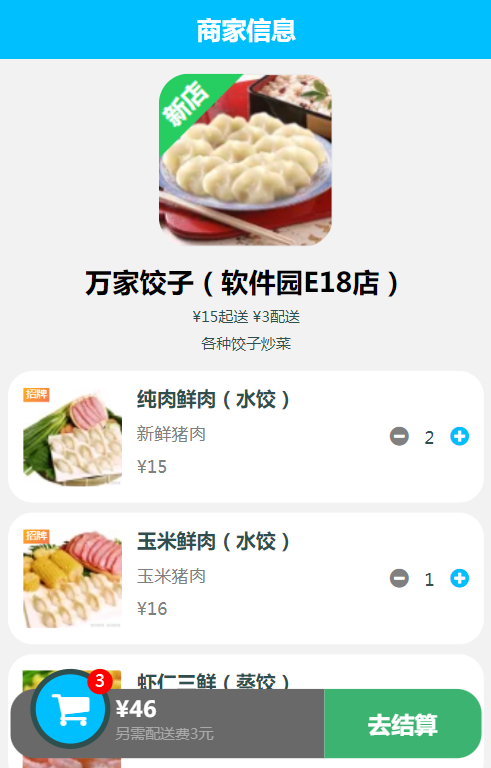
\includegraphics[width=0.4\textwidth]{businessInfo}
\caption{商家信息界面设计}\label{fig:businessInfo}
\vspace{\baselineskip}
\end{figure}
\subsubsection{功能按钮}
本软件商家信息功能按钮如表~\ref{tab:table4}~所示。
\begin{table}[htbp]
    \caption{饿了么外卖平台商家信息功能按钮}\label{tab:table4}
    \vspace{0.5em}\wuhao
    \begin{tabularx}{\textwidth}{lllX}
    \toprule[1.5pt]
    序号 & 按钮名称 & 功能 & 功能规则 \\ 
    \midrule[1pt]
    1 & 添加菜品 & 用户添加该菜品数量 & 点击将该菜品在购物车里的数量加1。 \\
    2 & 减少菜品 & 用户减少该菜品数量 & 点击将该菜品在购物车里的数量减1。 \\
    3 & 去结算 & 进入确认订单页面 & 点击会生成订单,跳转至确认订单页面。 \\
\bottomrule[1.5pt]
\end{tabularx}
\vspace{\baselineskip}
\end{table}

\subsection{确认订单}
当用户在商家信息页面中点击【去结算】按钮后,会跳转至确认订单页面。此页面展示了当前用户的送货地址、用户名称和手机号。在用户信息的下方显示了商家名称、购物车中所选择的菜品图片、菜品名称、菜品数量和配送费。在此页面的底部显示了总价格和【去支付】的按钮。
\subsubsection{界面设计}
本软件的确认订单界面设计如图~\ref{fig:order}~所示。
\begin{figure}[htbp]
\centering
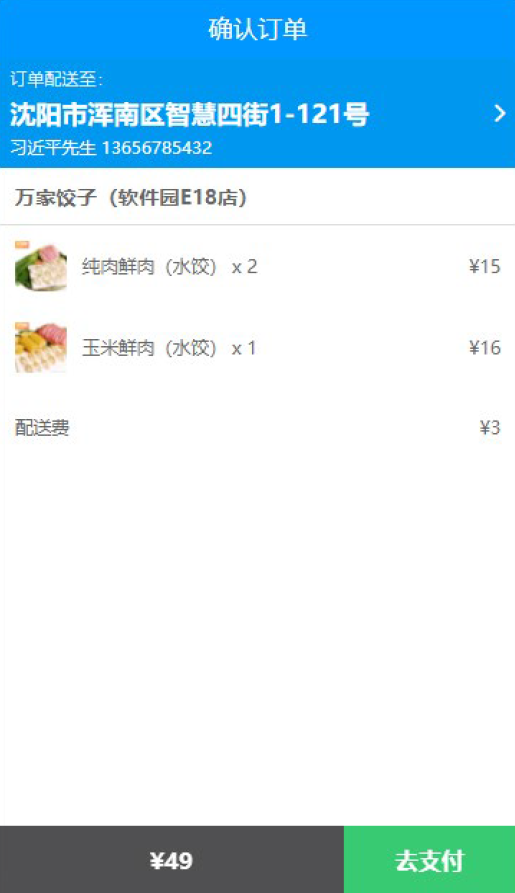
\includegraphics[width=0.4\textwidth]{order}
\caption{确认订单界面设计}\label{fig:order}
\vspace{\baselineskip}
\end{figure}
\subsubsection{功能按钮}
本软件确认订单功能按钮如表~\ref{tab:table5}~所示。
\begin{table}[htbp]
    \caption{饿了么外卖平台确认订单功能按钮}\label{tab:table5}
    \vspace{0.5em}\wuhao
    \begin{tabularx}{\textwidth}{lllX}
    \toprule[1.5pt]
    序号 & 按钮名称 & 功能 & 功能规则 \\ 
    \midrule[1pt]
    1 & 当前送货地址 & 用户选择送货地址 & 点击跳转至地址管理页面。 \\
    2 & 去支付 & 进入在线支付页面 & 点击跳转至在线支付页面。 \\
\bottomrule[1.5pt]
\end{tabularx}
\vspace{\baselineskip}
\end{table}

\subsection{在线支付}
当用户在确认订单页面中点击【去结算】按钮后,会跳转至确认订单页面。
\subsubsection{界面设计}
本软件的在线支付界面设计如图~\ref{fig:payment}~所示。
\begin{figure}[htbp]
\centering
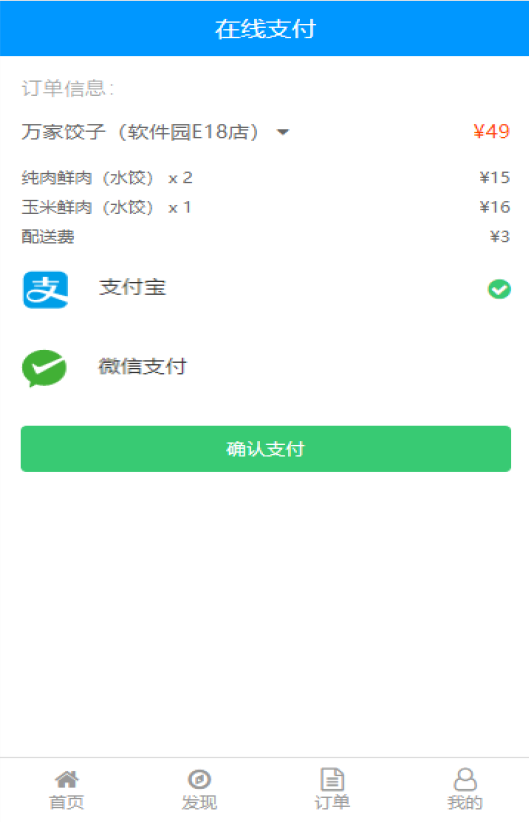
\includegraphics[width=0.4\textwidth]{payment}
\caption{在线支付界面设计}\label{fig:payment}
\vspace{\baselineskip}
\end{figure}
\subsubsection{功能按钮}
本软件在线支付功能按钮如表~\ref{tab:table6}~所示。
\begin{table}[htbp]
    \caption{饿了么外卖平台在线支付功能按钮}\label{tab:table6}
    \vspace{0.5em}\wuhao
    \begin{tabularx}{\textwidth}{lllX}
    \toprule[1.5pt]
    序号 & 按钮名称 & 功能 & 功能规则 \\ 
    \midrule[1pt]
    1 & 箭头 & 用户展开订单明细 & 点击展开已生成的订单明细,包括菜品的数量和价格。 \\
    2 & 选择支付方式 & 用户选择第三方的支付方式 & 点击选择任一第三方支付方式。 \\
    3 & 确认支付 & 用户支付订单 & 点击完成点餐流程。 \\
    4 & 首页 & 进入首页 & 点击跳转至首页。 \\
    5 & 订单 & 进入历史订单 & 点击跳转至历史订单页面。 \\
    6 & 我的 & 进入用户信息 & 点击跳转至用户信息页面。 \\
\bottomrule[1.5pt]
\end{tabularx}
\vspace{\baselineskip}
\end{table}

\subsection{用户登录}
此页面为用户登录的页面。用户需要输入手机号和密码,若两者正确无误则登陆成功并跳转至上一个页面,否则服务器将会提示信息错误。
\subsubsection{界面设计}
本软件的用户登录界面设计如图~\ref{fig:login}~所示。
\begin{figure}[htbp]
\centering
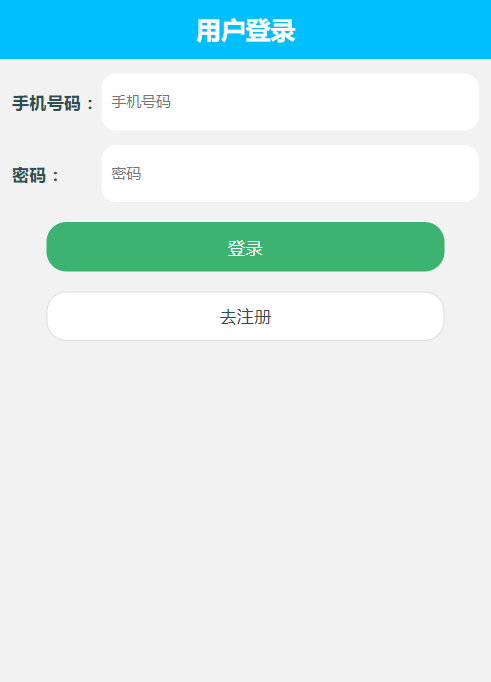
\includegraphics[width=0.4\textwidth]{login}
\caption{用户登录界面设计}\label{fig:login}
\vspace{\baselineskip}
\end{figure}
\subsubsection{功能按钮}
本软件用户登录功能按钮如表~\ref{tab:table7}~所示。
\begin{table}[htbp]
    \caption{饿了么外卖平台用户登录功能按钮}\label{tab:table7}
    \vspace{0.5em}\wuhao
    \begin{tabularx}{\textwidth}{lllX}
    \toprule[1.5pt]
    序号 & 按钮名称 & 功能 & 功能规则 \\ 
    \midrule[1pt]
    1 & 登录 & 用户登录 & 若手登陆成功则跳转至上一个页面,否则服务器将会显示错误提示。 \\
    2 & 去注册 & 用户注册 & 点击跳转至用户注册页面。 \\
    3 & 首页 & 进入首页 & 点击跳转至首页。 \\
    4 & 订单 & 进入历史订单 & 点击跳转至历史订单页面。 \\
    5 & 我的 & 进入用户信息 & 点击跳转至用户信息页面。 \\
\bottomrule[1.5pt]
\end{tabularx}
\vspace{\baselineskip}
\end{table}

\subsection{用户注册}
此页面为用户注册的页面。用户需要输入手机号、两次相同的密码、用户姓名以及选择性别。若手机号、密码和用户名都符合要求,则注册成功并跳转至登陆页面,否则服务器将会提示信息错误。
\subsubsection{界面设计}
本软件的用户注册界面设计如图~\ref{fig:register}~所示。
\begin{figure}[htbp]
\centering
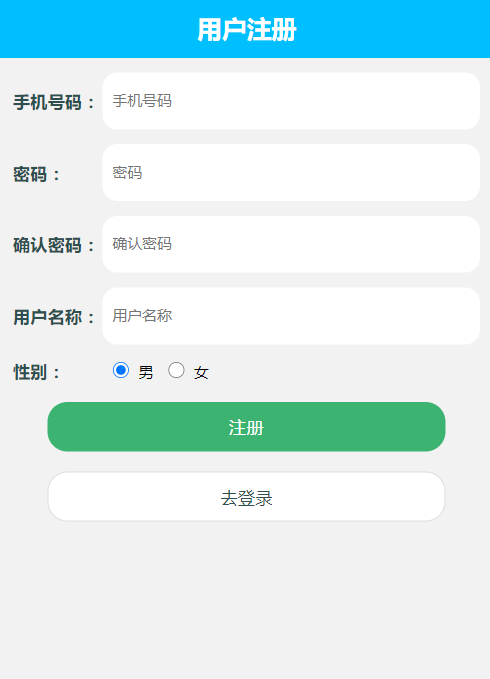
\includegraphics[width=0.4\textwidth]{register}
\caption{用户注册界面设计}\label{fig:register}
\vspace{\baselineskip}
\end{figure}
\subsubsection{功能按钮}
本软件用户注册功能按钮如表~\ref{tab:table8}~所示。
\begin{table}[htbp]
    \caption{饿了么外卖平台用户注册功能按钮}\label{tab:table8}
    \vspace{0.5em}\wuhao
    \begin{tabularx}{\textwidth}{lllX}
    \toprule[1.5pt]
    序号 & 按钮名称 & 功能 & 功能规则 \\ 
    \midrule[1pt]
    1 & 性别 & 用户选择性别 & 点击选择任一性别。 \\
    2 & 注册 & 用户注册 & 若注册成功则跳转至登陆页面,否则服务器将显示错误提示。 \\
    3 & 首页 & 进入首页 & 点击跳转至首页。 \\
    4 & 订单 & 进入历史订单 & 点击跳转至历史订单页面。 \\
    5 & 我的 & 进入用户信息 & 点击跳转至用户信息页面。 \\
\bottomrule[1.5pt]
\end{tabularx}
\vspace{\baselineskip}
\end{table}

\subsection{历史订单}
历史订单页面展示了用户之前所生成的全部订单,未支付的订单会显示在页面的上方,已支付的订单则会显示在页面的下方。
\subsubsection{界面设计}
本软件的历史订单界面设计如图~\ref{fig:orderList}~所示。
\begin{figure}[htbp]
\centering
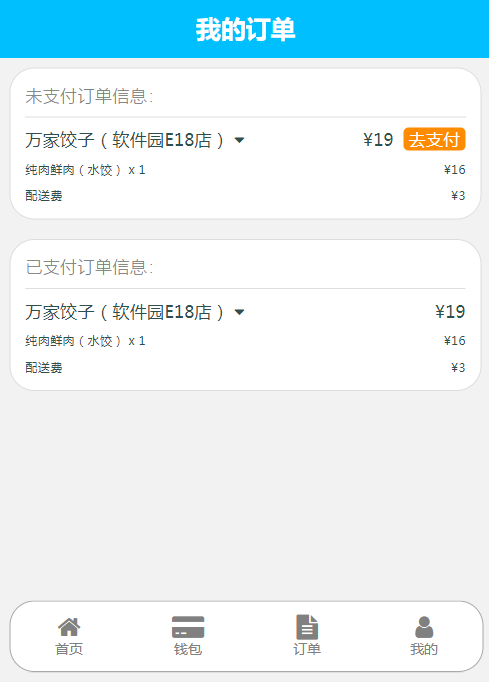
\includegraphics[width=0.4\textwidth]{orderList}
\caption{历史订单界面设计}\label{fig:orderList}
\vspace{\baselineskip}
\end{figure}
\subsubsection{功能按钮}
本软件历史订单功能按钮如表~\ref{tab:table9}~所示。
\begin{table}[htbp]
    \caption{饿了么外卖平台历史订单功能按钮}\label{tab:table9}
    \vspace{0.5em}\wuhao
    \begin{tabularx}{\textwidth}{lllX}
    \toprule[1.5pt]
    序号 & 按钮名称 & 功能 & 功能规则 \\ 
    \midrule[1pt]
    1 & 箭头 & 用户展开订单明细 & 点击展开已生成的订单明细,包括菜品的数量和价格。 \\
    2 & 去支付 & 用户支付未支付的订单 & 点击跳转至未支付的订单页面。 \\
    3 & 首页 & 进入首页 & 点击跳转至首页。 \\
    4 & 订单 & 刷新页面 & 点击跳转至历史订单页面。 \\
    5 & 我的 & 进入用户信息 & 点击跳转至用户信息页面。 \\
\bottomrule[1.5pt]
\end{tabularx}
\vspace{\baselineskip}
\end{table}

\subsection{地址管理}
当用户在首页或在确认订单页面点击送货地址按钮时,会跳转到此页面。此页面显示了用户的所有送货地址。
\subsubsection{界面设计}
本软件的地址管理界面设计如图~\ref{fig:userAddress}~所示。
\begin{figure}[htbp]
\centering
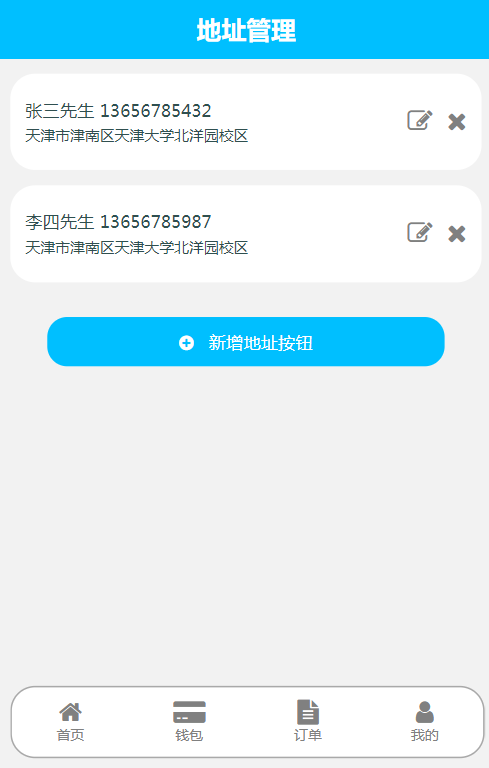
\includegraphics[width=0.4\textwidth]{userAddress}
\caption{地址管理界面设计}\label{fig:userAddress}
\vspace{\baselineskip}
\end{figure}
\subsubsection{功能按钮}
本软件地址管理功能按钮如表~\ref{tab:table10}~所示。
\begin{table}[htbp]
    \caption{饿了么外卖平台地址管理功能按钮}\label{tab:table10}
    \vspace{0.5em}\wuhao
    \begin{tabularx}{\textwidth}{lllX}
    \toprule[1.5pt]
    序号 & 按钮名称 & 功能 & 功能规则 \\ 
    \midrule[1pt]
    1 & 送货地址 & 用户选择该送货地址 & 点击选择该送货地址,并跳转至上一个页面。 \\
    2 & 编辑图标 & 用户编辑该送货地址 & 点击跳转至编辑送货地址页面。 \\
    3 & 打叉图标 & 用户删除该送货地址 & 点击删除该送货地址,地址管理页面减少该送货地址。 \\
    4 & 新增收货地址 & 用户添加送货地址 & 点击跳转至新增送货地址页面。 \\
    5 & 首页 & 进入首页 & 点击跳转至首页。 \\
    6 & 订单 & 进入历史订单 & 点击跳转至历史订单页面。 \\
    7 & 我的 & 进入用户信息 & 点击跳转至用户信息页面。 \\
\bottomrule[1.5pt]
\end{tabularx}
\vspace{\baselineskip}
\end{table}

\subsection{新增送货地址}
用户在此页面添加新的送货地址。填写完成后,点击保存按钮跳转至地址管理页面。
\subsubsection{界面设计}
本软件的新增送货地址界面设计如图~\ref{fig:addUserAddress}~所示。
\begin{figure}[htbp]
\centering
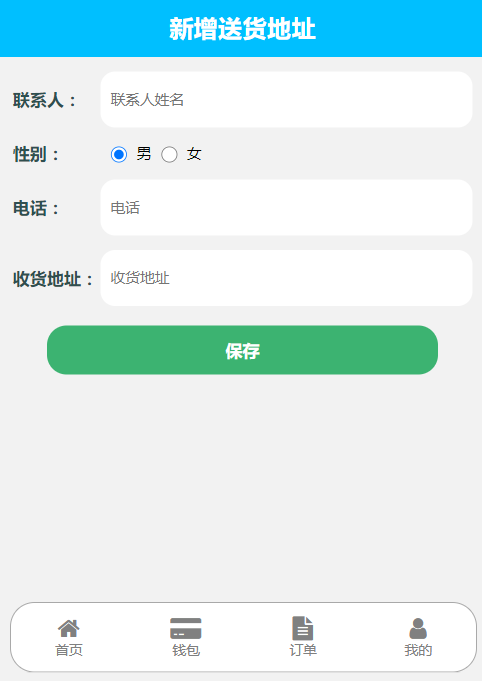
\includegraphics[width=0.4\textwidth]{addUserAddress}
\caption{新增送货地址界面设计}\label{fig:addUserAddress}
\vspace{\baselineskip}
\end{figure}
\subsubsection{功能按钮}
本软件新增送货地址功能按钮如表~\ref{tab:table11}~所示。
\begin{table}[htbp]
    \caption{饿了么外卖平台新增送货地址功能按钮}\label{tab:table11}
    \vspace{0.5em}\wuhao
    \begin{tabularx}{\textwidth}{lllX}
    \toprule[1.5pt]
    序号 & 按钮名称 & 功能 & 功能规则 \\ 
    \midrule[1pt]
    1 & 性别 & 用户选择性别 & 点击选择任一性别。 \\
    2 & 保存 & 用户保存当前送货地址 & 点击跳转至地址管理页面。 \\
    3 & 首页 & 进入首页 & 点击跳转至首页。 \\
    4 & 订单 & 进入历史订单 & 点击跳转至历史订单页面。 \\
    5 & 我的 & 进入用户信息 & 点击跳转至用户信息页面。 \\
\bottomrule[1.5pt]
\end{tabularx}
\vspace{\baselineskip}
\end{table}

\subsection{编辑地址}
用户在此页面编辑已选择的送货地址。填写完成后,点击保存按钮跳转至地址管理页面。
\subsubsection{界面设计}
本软件的编辑送货地址界面设计如图~\ref{fig:editUserAddress}~所示。
\begin{figure}[htbp]
\centering
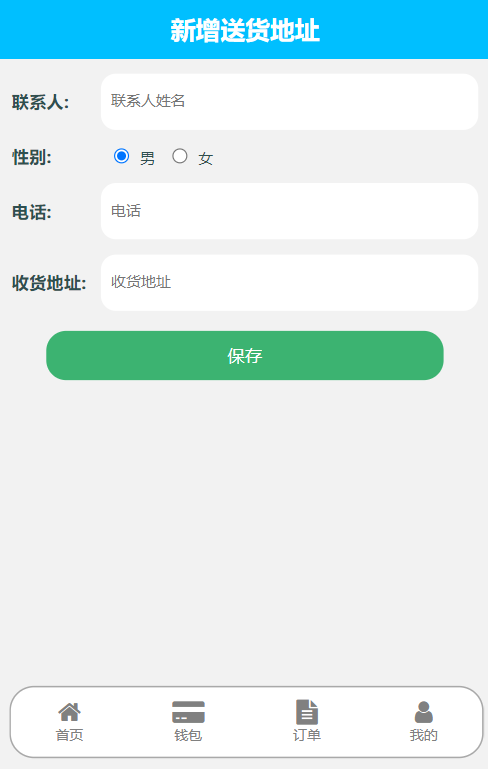
\includegraphics[width=0.4\textwidth]{editUserAddress}
\caption{编辑送货地址界面设计}\label{fig:editUserAddress}
\vspace{\baselineskip}
\end{figure}
\subsubsection{功能按钮}
本软件编辑送货地址功能按钮如表~\ref{tab:table12}~所示。
\begin{table}[htbp]
    \caption{饿了么外卖平台编辑送货地址功能按钮}\label{tab:table12}
    \vspace{0.5em}\wuhao
    \begin{tabularx}{\textwidth}{lllX}
    \toprule[1.5pt]
    序号 & 按钮名称 & 功能 & 功能规则 \\ 
    \midrule[1pt]
    1 & 性别 & 用户选择性别 & 点击选择任一性别。 \\
    2 & 保存 & 用户保存当前送货地址 & 点击跳转至地址管理页面。 \\
    3 & 首页 & 进入首页 & 点击跳转至首页。 \\
    4 & 订单 & 进入历史订单 & 点击跳转至历史订单页面。 \\
    5 & 我的 & 进入用户信息 & 点击跳转至用户信息页面。 \\
\bottomrule[1.5pt]
\end{tabularx}
\vspace{\baselineskip}
\end{table}

\subsection{个人信息}
个人信息页面显示当前用户的图片和名称。用户可以在此页面修改用户名和密码、跳转至地址管理页面以及退出登录。
\subsubsection{界面设计}
本软件的个人信息界面设计如图~\ref{fig:profile}~所示。
\begin{figure}[htbp]
\centering
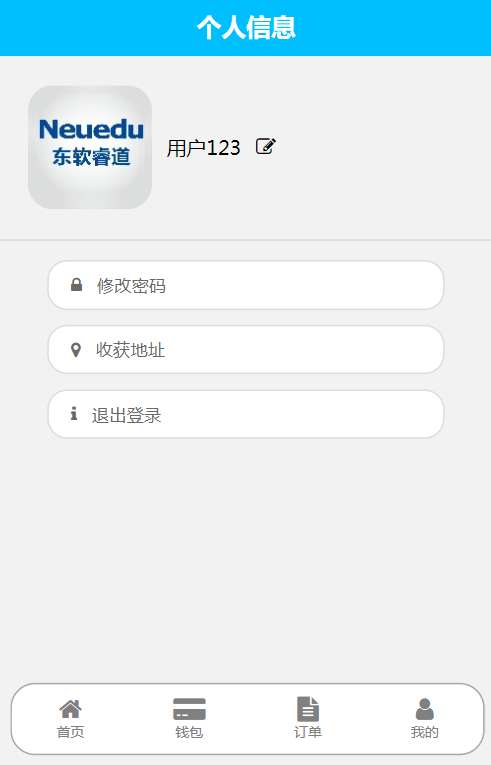
\includegraphics[width=0.4\textwidth]{profile}
\caption{个人信息界面设计}\label{fig:profile}
\vspace{\baselineskip}
\end{figure}
\subsubsection{功能按钮}
本软件编辑送货地址功能按钮如表~\ref{tab:table13}~所示。
\begin{table}[htbp]
    \caption{饿了么外卖平台编辑送货地址功能按钮}\label{tab:table13}
    \vspace{0.5em}\wuhao
    \begin{tabularx}{\textwidth}{lllX}
    \toprule[1.5pt]
    序号 & 按钮名称 & 功能 & 功能规则 \\ 
    \midrule[1pt]
    1 & 编辑图标 & 进入更新用户名页面 & 点击跳转至更新用户名页面。 \\
    2 & 修改密码 & 进入更新密码页面 & 点击跳转至更新密码页面。 \\
    3 & 收货地址 & 进入地址管理页面 & 点击跳转至地址管理页面。 \\
    4 & 退出登录 & 进入首页 & 点击退出登录,跳转至首页。 \\
    5 & 首页 & 进入首页 & 点击跳转至首页。 \\
    6 & 订单 & 进入历史订单页面 & 点击跳转至历史订单页面。 \\
    7 & 我的 & 刷新页面 & 点击跳转至用户信息页面。 \\
\bottomrule[1.5pt]
\end{tabularx}
\vspace{\baselineskip}
\end{table}

\subsection{更新用户名}
用户在此页面更新用户名。填写完成后,点击保存按钮跳转至个人信息页面。
\subsubsection{界面设计}
本软件的更新用户名界面设计如图~\ref{fig:updateUserName}~所示。
\begin{figure}[htbp]
\centering
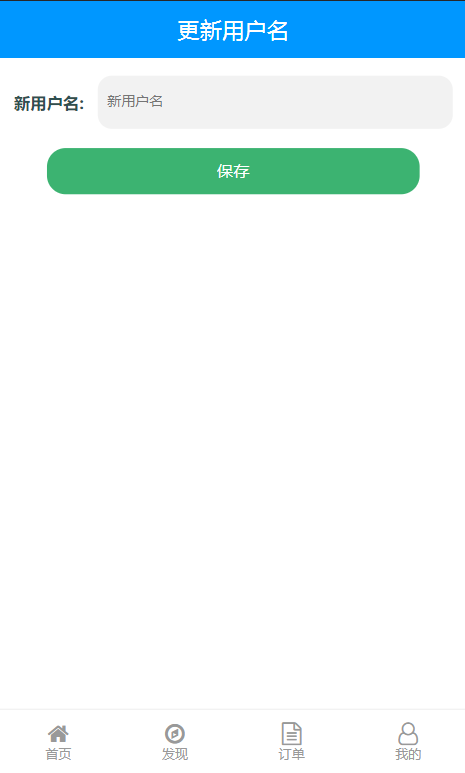
\includegraphics[width=0.4\textwidth]{updateUserName}
\caption{更新用户名界面设计}\label{fig:updateUserName}
\vspace{\baselineskip}
\end{figure}
\subsubsection{功能按钮}
本软件更新用户名功能按钮如表~\ref{tab:table14}~所示。
\begin{table}[htbp]
    \caption{饿了么外卖平台更新用户名功能按钮}\label{tab:table14}
    \vspace{0.5em}\wuhao
    \begin{tabularx}{\textwidth}{lllX}
    \toprule[1.5pt]
    序号 & 按钮名称 & 功能 & 功能规则 \\ 
    \midrule[1pt]
    1 & 保存 & 用户保存当前用户名 & 点击跳转至个人信息页面。 \\
    2 & 首页 & 进入首页 & 点击跳转至首页。 \\
    3 & 订单 & 进入历史订单页面 & 点击跳转至历史订单页面。 \\
    4 & 我的 & 刷新页面 & 点击跳转至用户信息页面。 \\
\bottomrule[1.5pt]
\end{tabularx}
\vspace{\baselineskip}
\end{table}

\subsection{更新密码}
用户在此页面更新密码。填写完成后,点击保存按钮跳转至个人信息页面。
\subsubsection{界面设计}
本软件的更新密码界面设计如图~\ref{fig:updateUserPassword}~所示。
\begin{figure}[htbp]
\centering
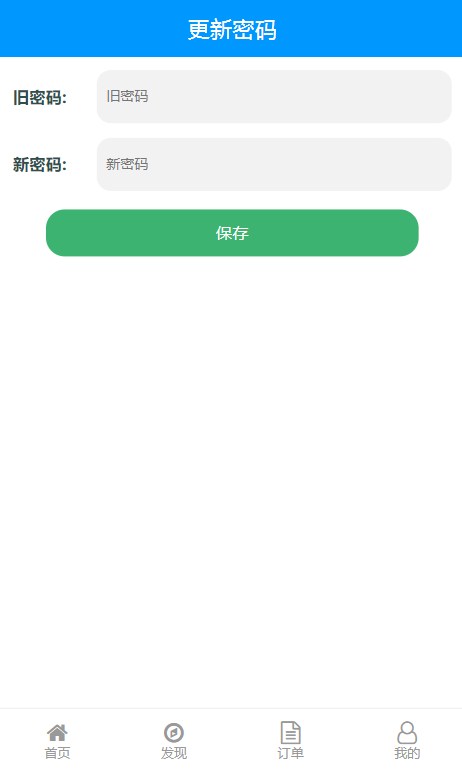
\includegraphics[width=0.4\textwidth]{updateUserPassword}
\caption{更新密码界面设计}\label{fig:updateUserPassword}
\vspace{\baselineskip}
\end{figure}
\subsubsection{功能按钮}
本软件更新密码功能按钮如表~\ref{tab:table15}~所示。
\begin{table}[htbp]
    \caption{饿了么外卖平台更新密码功能按钮}\label{tab:table15}
    \vspace{0.5em}\wuhao
    \begin{tabularx}{\textwidth}{lllX}
    \toprule[1.5pt]
    序号 & 按钮名称 & 功能 & 功能规则 \\ 
    \midrule[1pt]
    1 & 保存 & 用户保存当前密码 & 点击跳转至个人信息页面。 \\
    2 & 首页 & 进入首页 & 点击跳转至首页。 \\
    3 & 订单 & 进入历史订单页面 & 点击跳转至历史订单页面。 \\
    4 & 我的 & 刷新页面 & 点击跳转至用户信息页面。 \\
\bottomrule[1.5pt]
\end{tabularx}
\vspace{\baselineskip}
\end{table} %项目需求
	\chapter{项目设计} %项目设计
	\chapter{项目测试} %项目测试
	\chapter{项目部署} %项目部署
	\chapter{项目开发过程} %项目开发过程
	\chapter{项目特色之处} %项目特色之处
	\chapter{项目中遇到的问题及解决方法} %项目中遇到的问题及解决方法
	\chapter{附件}
\section{新技术学习视频截图}

\begin{figure}[htbp]
    \centering
    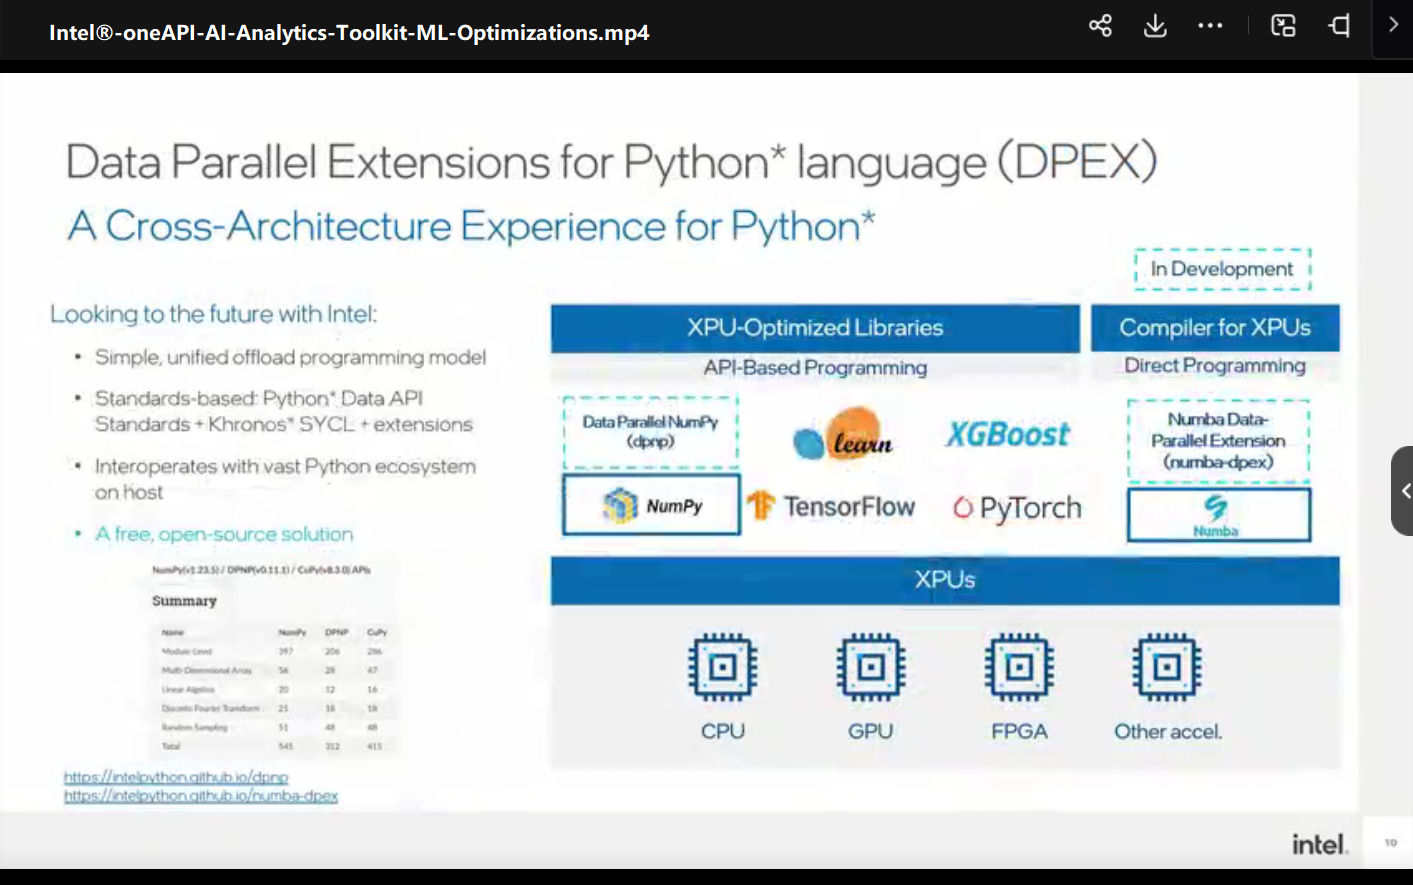
\includegraphics[width=0.7\textwidth]{3021244187_AI}
    \caption{3021244187 易东廷}\label{fig:3021244187_AI}
    \vspace{\baselineskip}
\end{figure}
\begin{figure}[htbp]
    \centering
    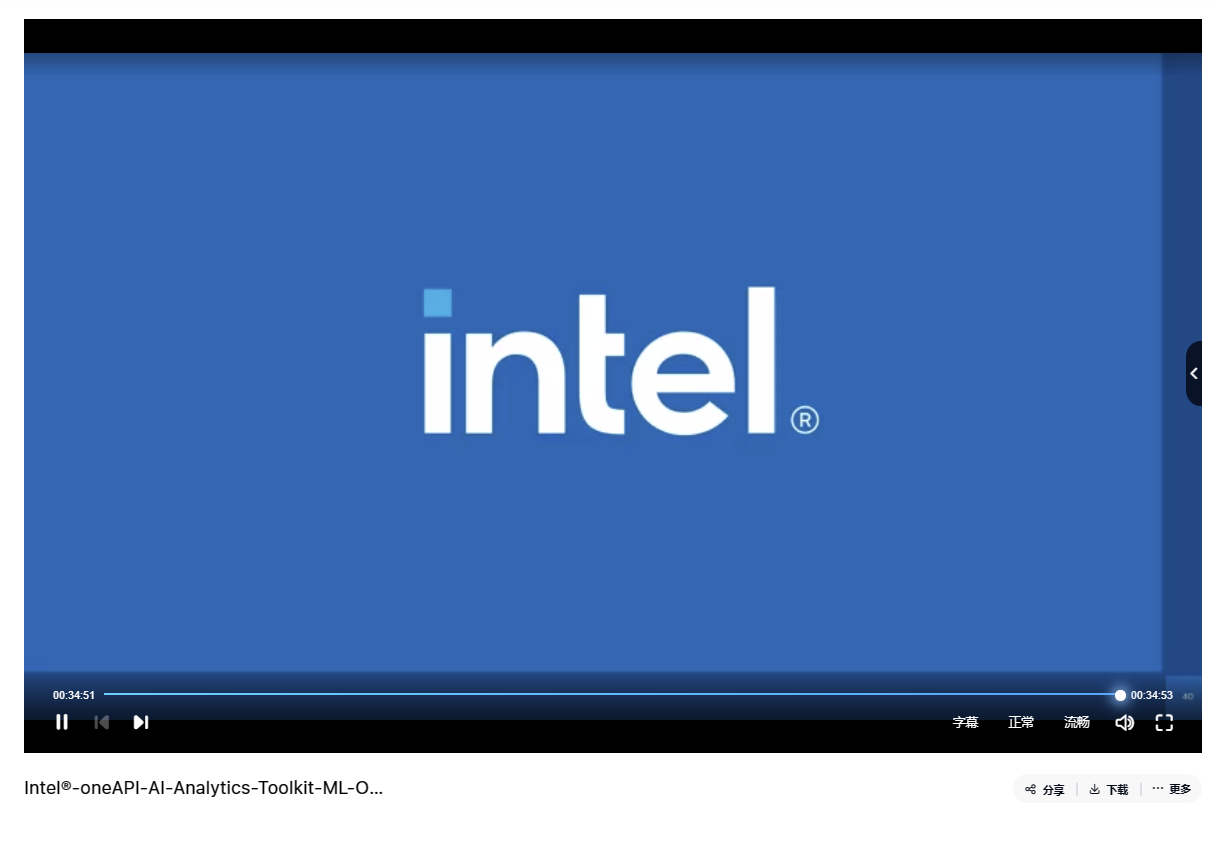
\includegraphics[width=0.8\textwidth]{3021210045_AI}
    \caption{3021210045 张中天}\label{fig:3021210045_AI}
    \vspace{\baselineskip}
\end{figure}
\begin{figure}[htbp]
    \centering
    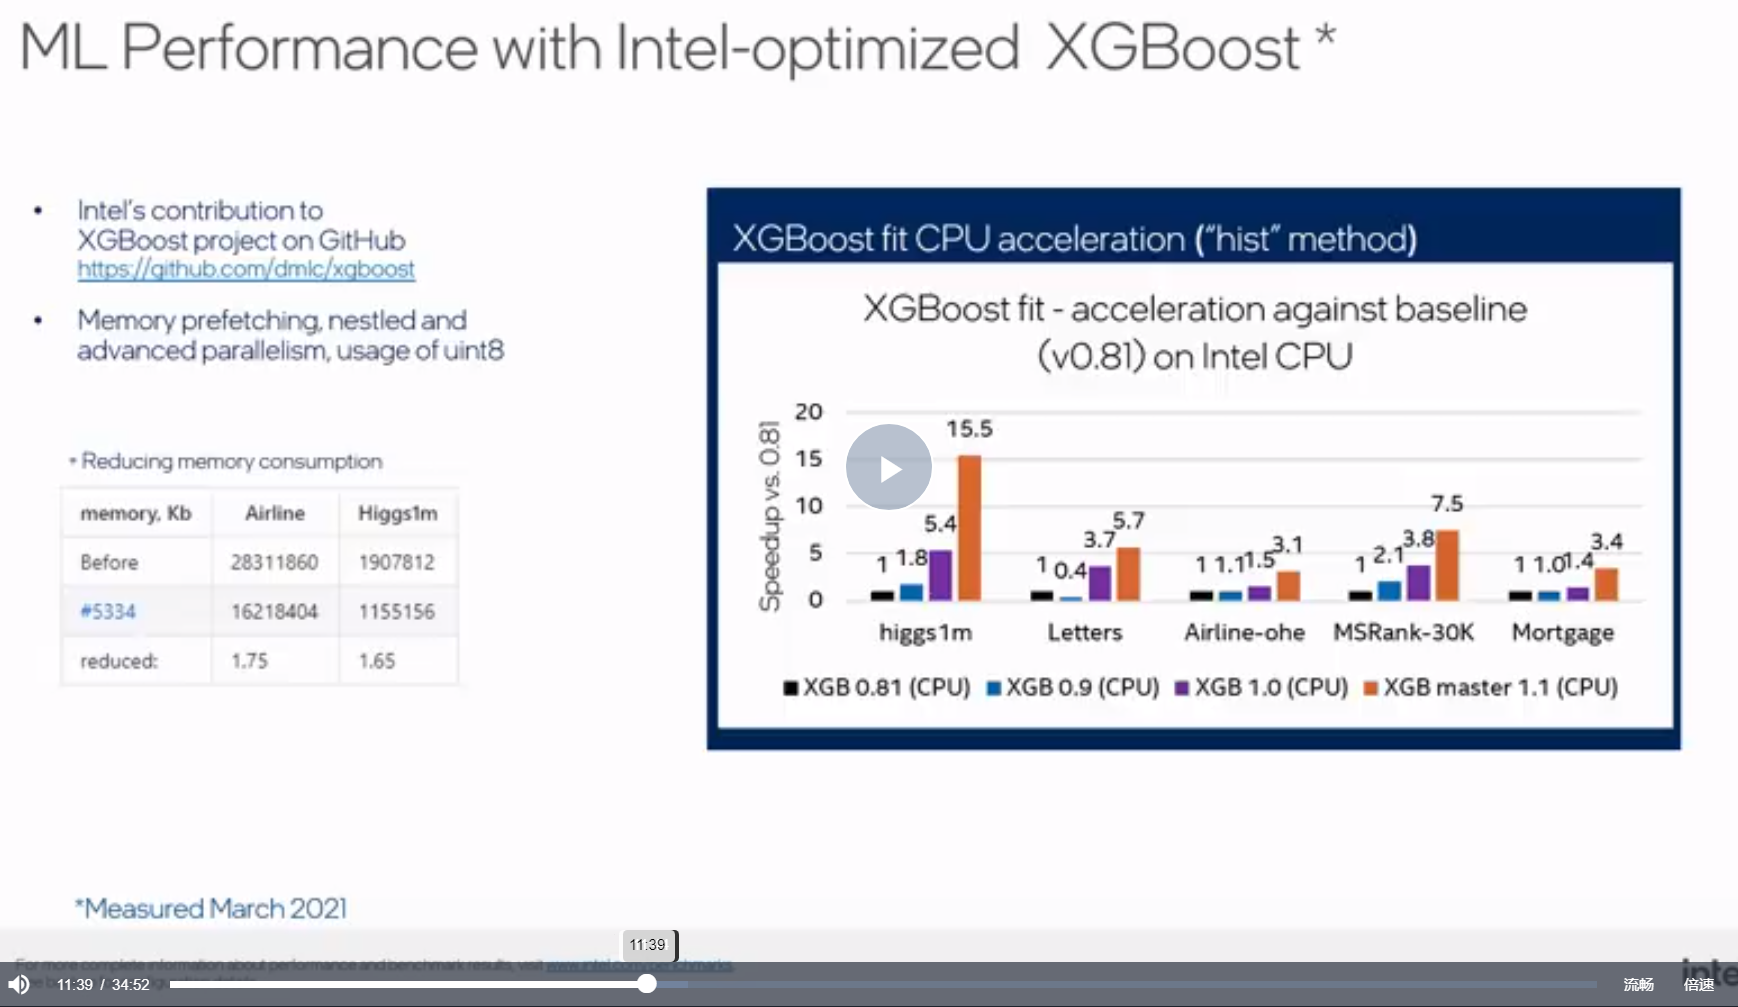
\includegraphics[width=0.8\textwidth]{3021244259_AI}
    \caption{3021244259 张梅梅}\label{fig:3021244259_AI}
    \vspace{\baselineskip}
\end{figure}
\begin{figure}[htbp]
    \centering
    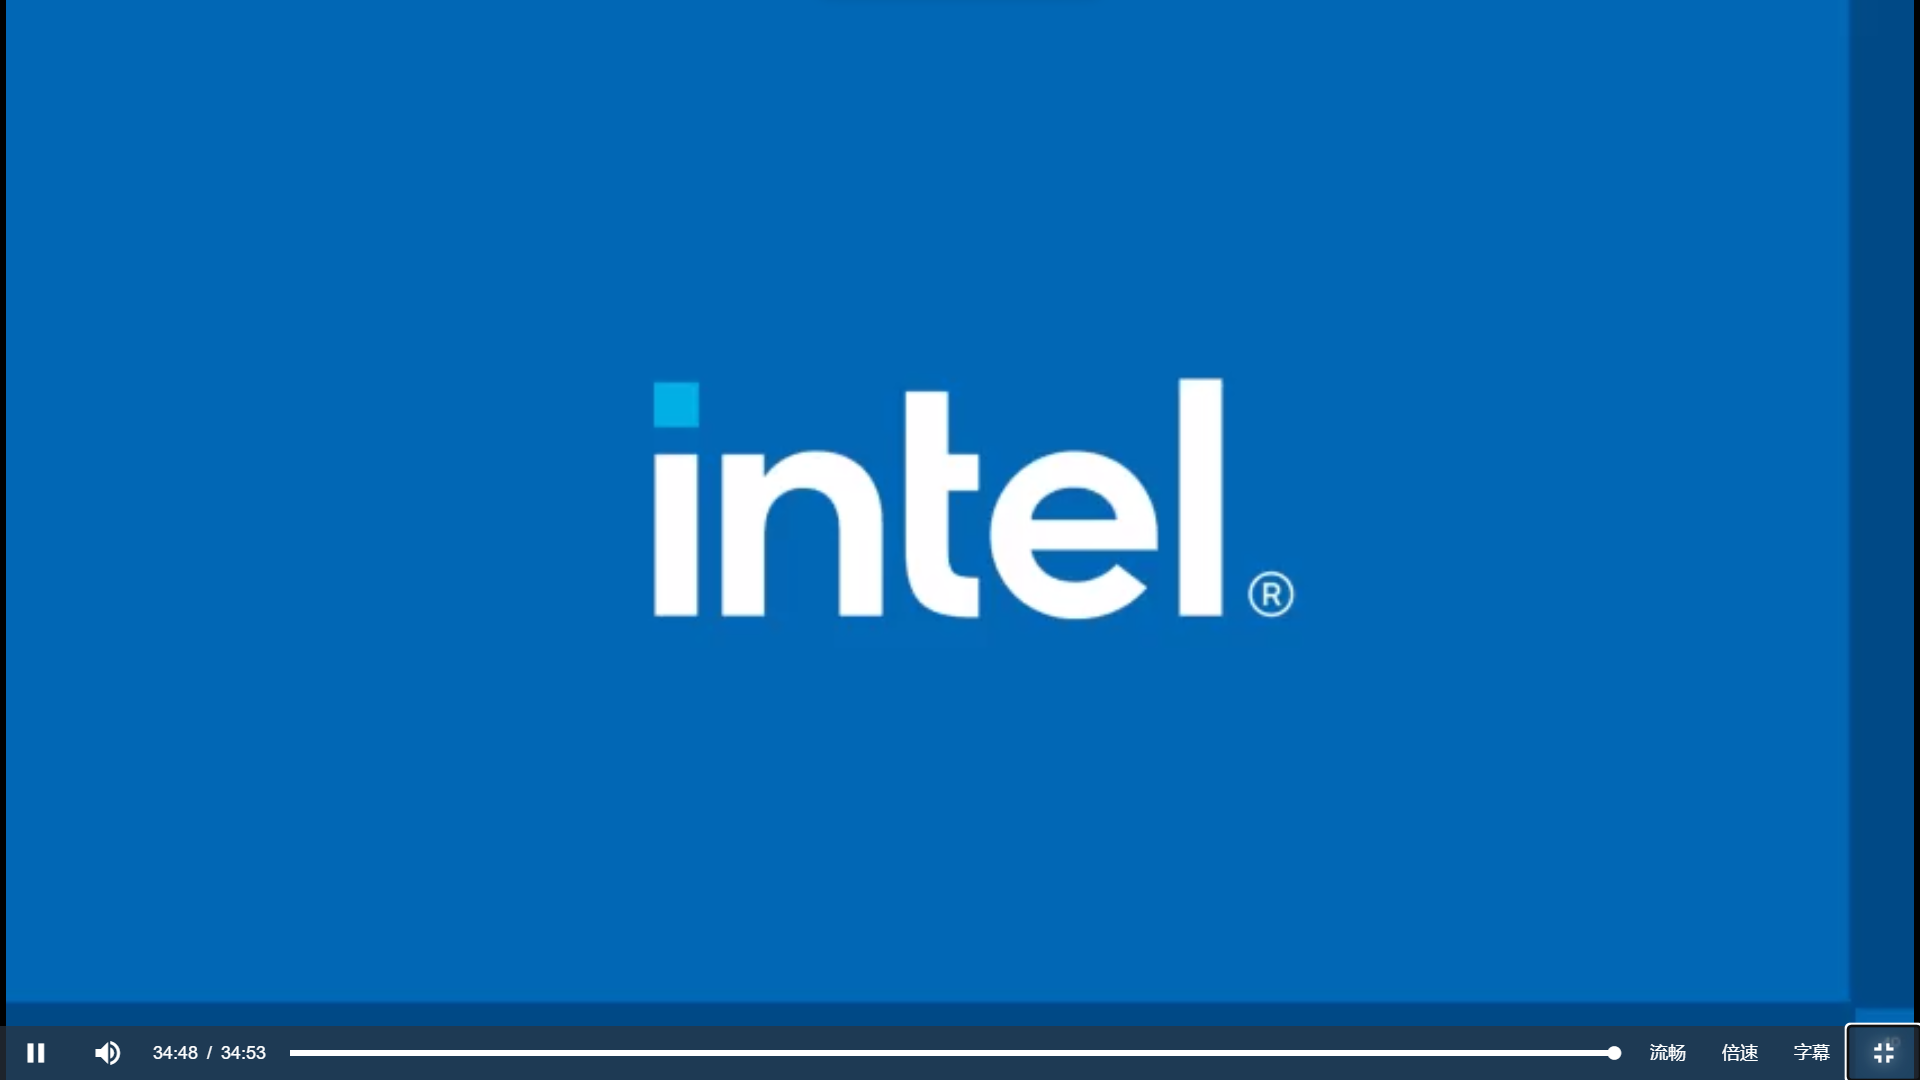
\includegraphics[width=0.8\textwidth]{6321012105_AI}
    \caption{6321012105 杜伟乐}\label{fig:6321012105_AI}
    \vspace{\baselineskip}
\end{figure}

\begin{figure}[htbp]
    \centering
    \begin{minipage}{0.4\textwidth}
        \centering
        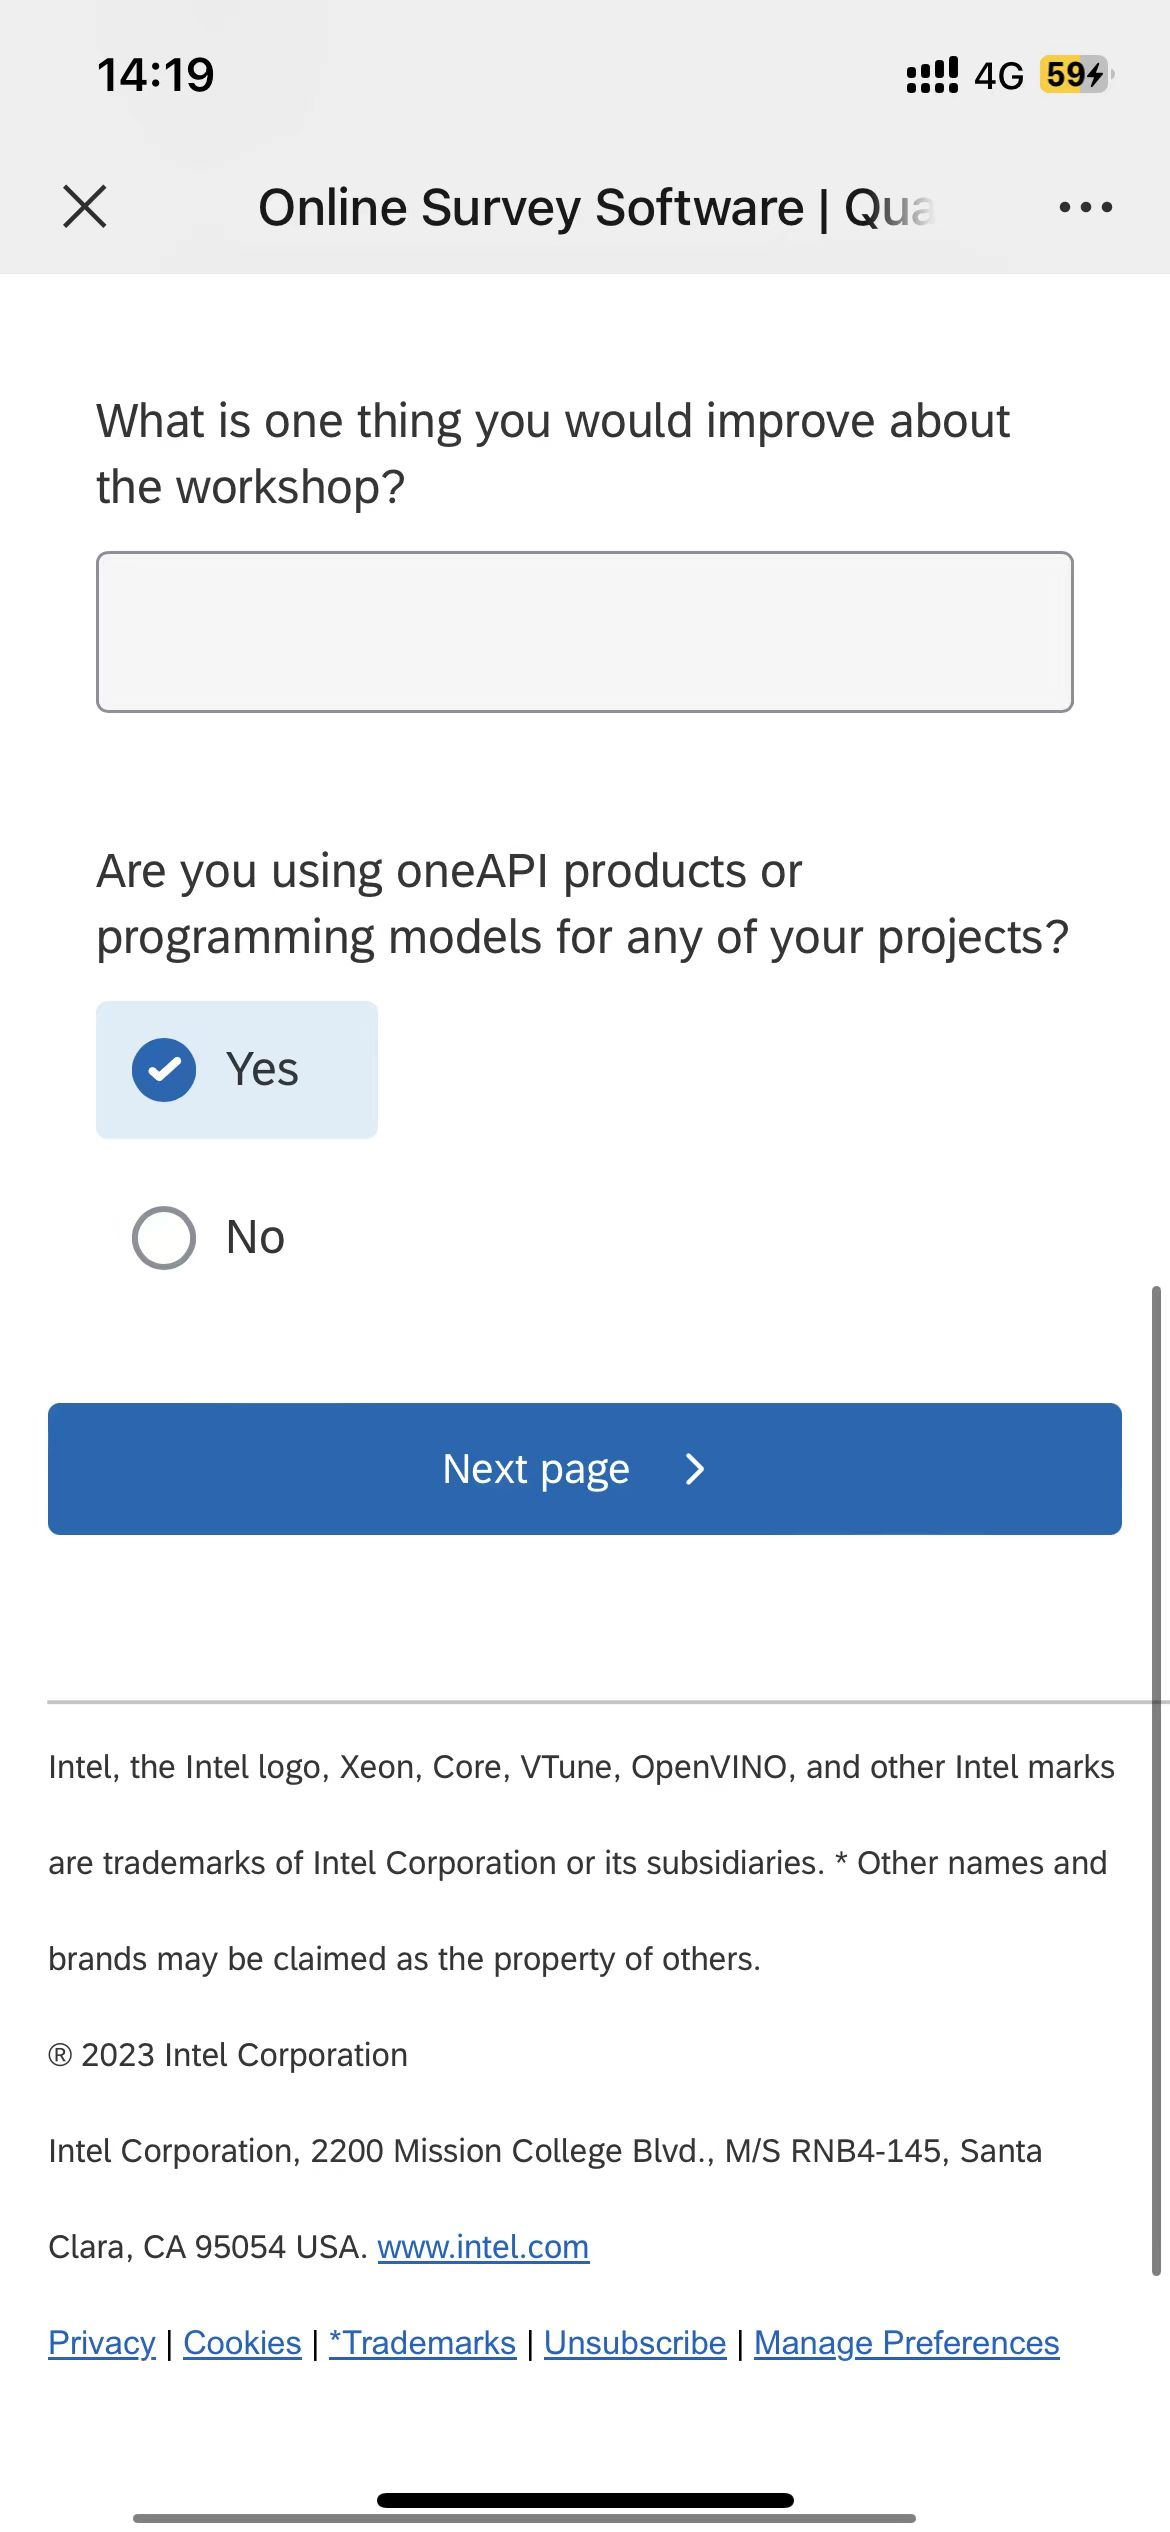
\includegraphics[width=\textwidth]{3021244187_form}
        \caption{3021244187 易东廷}\label{fig:3021244187_form}
    \end{minipage}
    \begin{minipage}{0.4\textwidth}
        \centering
        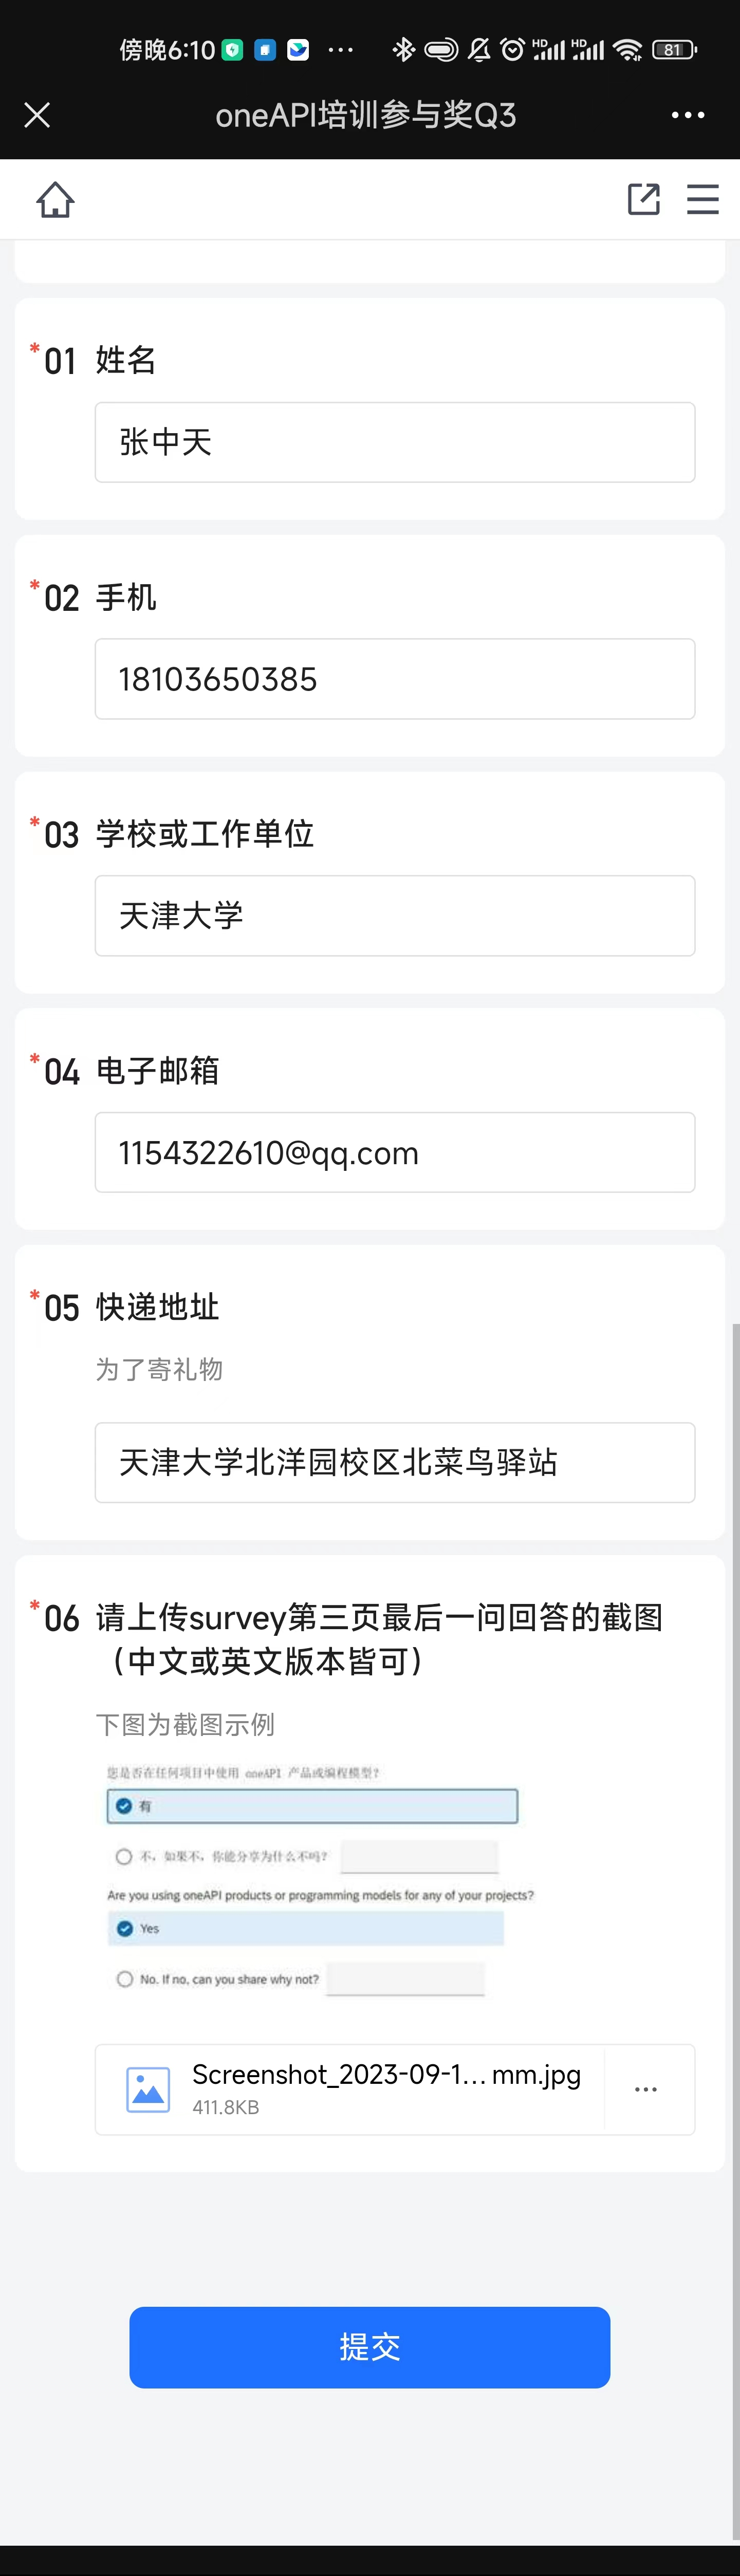
\includegraphics[width=\textwidth]{3021210045_form}
        \caption{3021210045 张中天}\label{fig:3021210045_form}
    \end{minipage}
\end{figure}
\begin{figure}[htbp]
    \centering
    \begin{minipage}{0.4\textwidth}
        \centering
        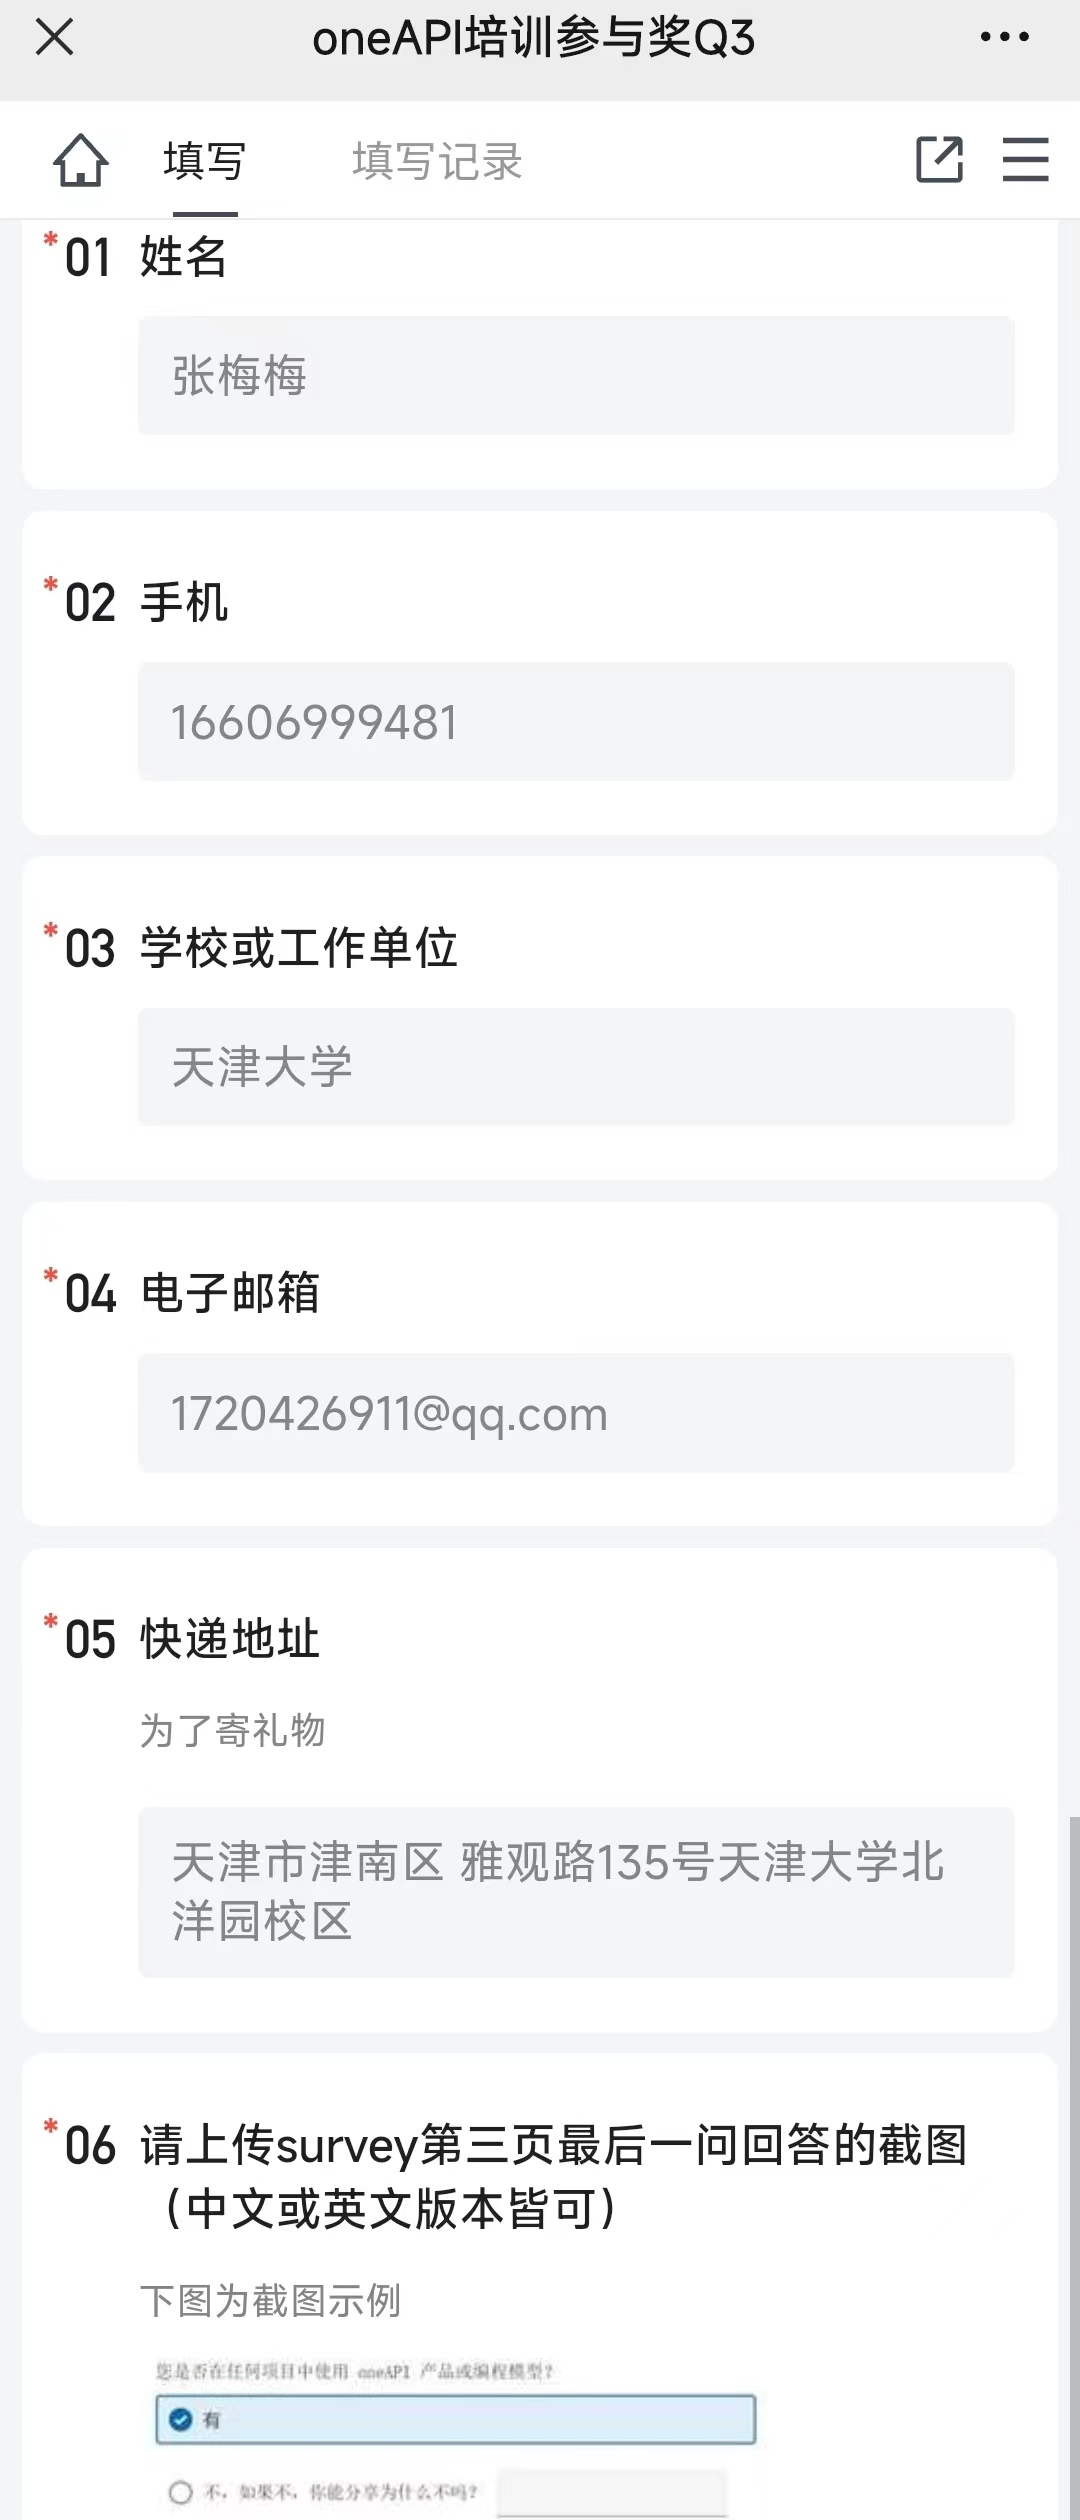
\includegraphics[width=\textwidth]{3021244259_form}
        \caption{3021244259 张梅梅}\label{fig:3021244259_form}
    \end{minipage}
    \begin{minipage}{0.4\textwidth}
        \centering
        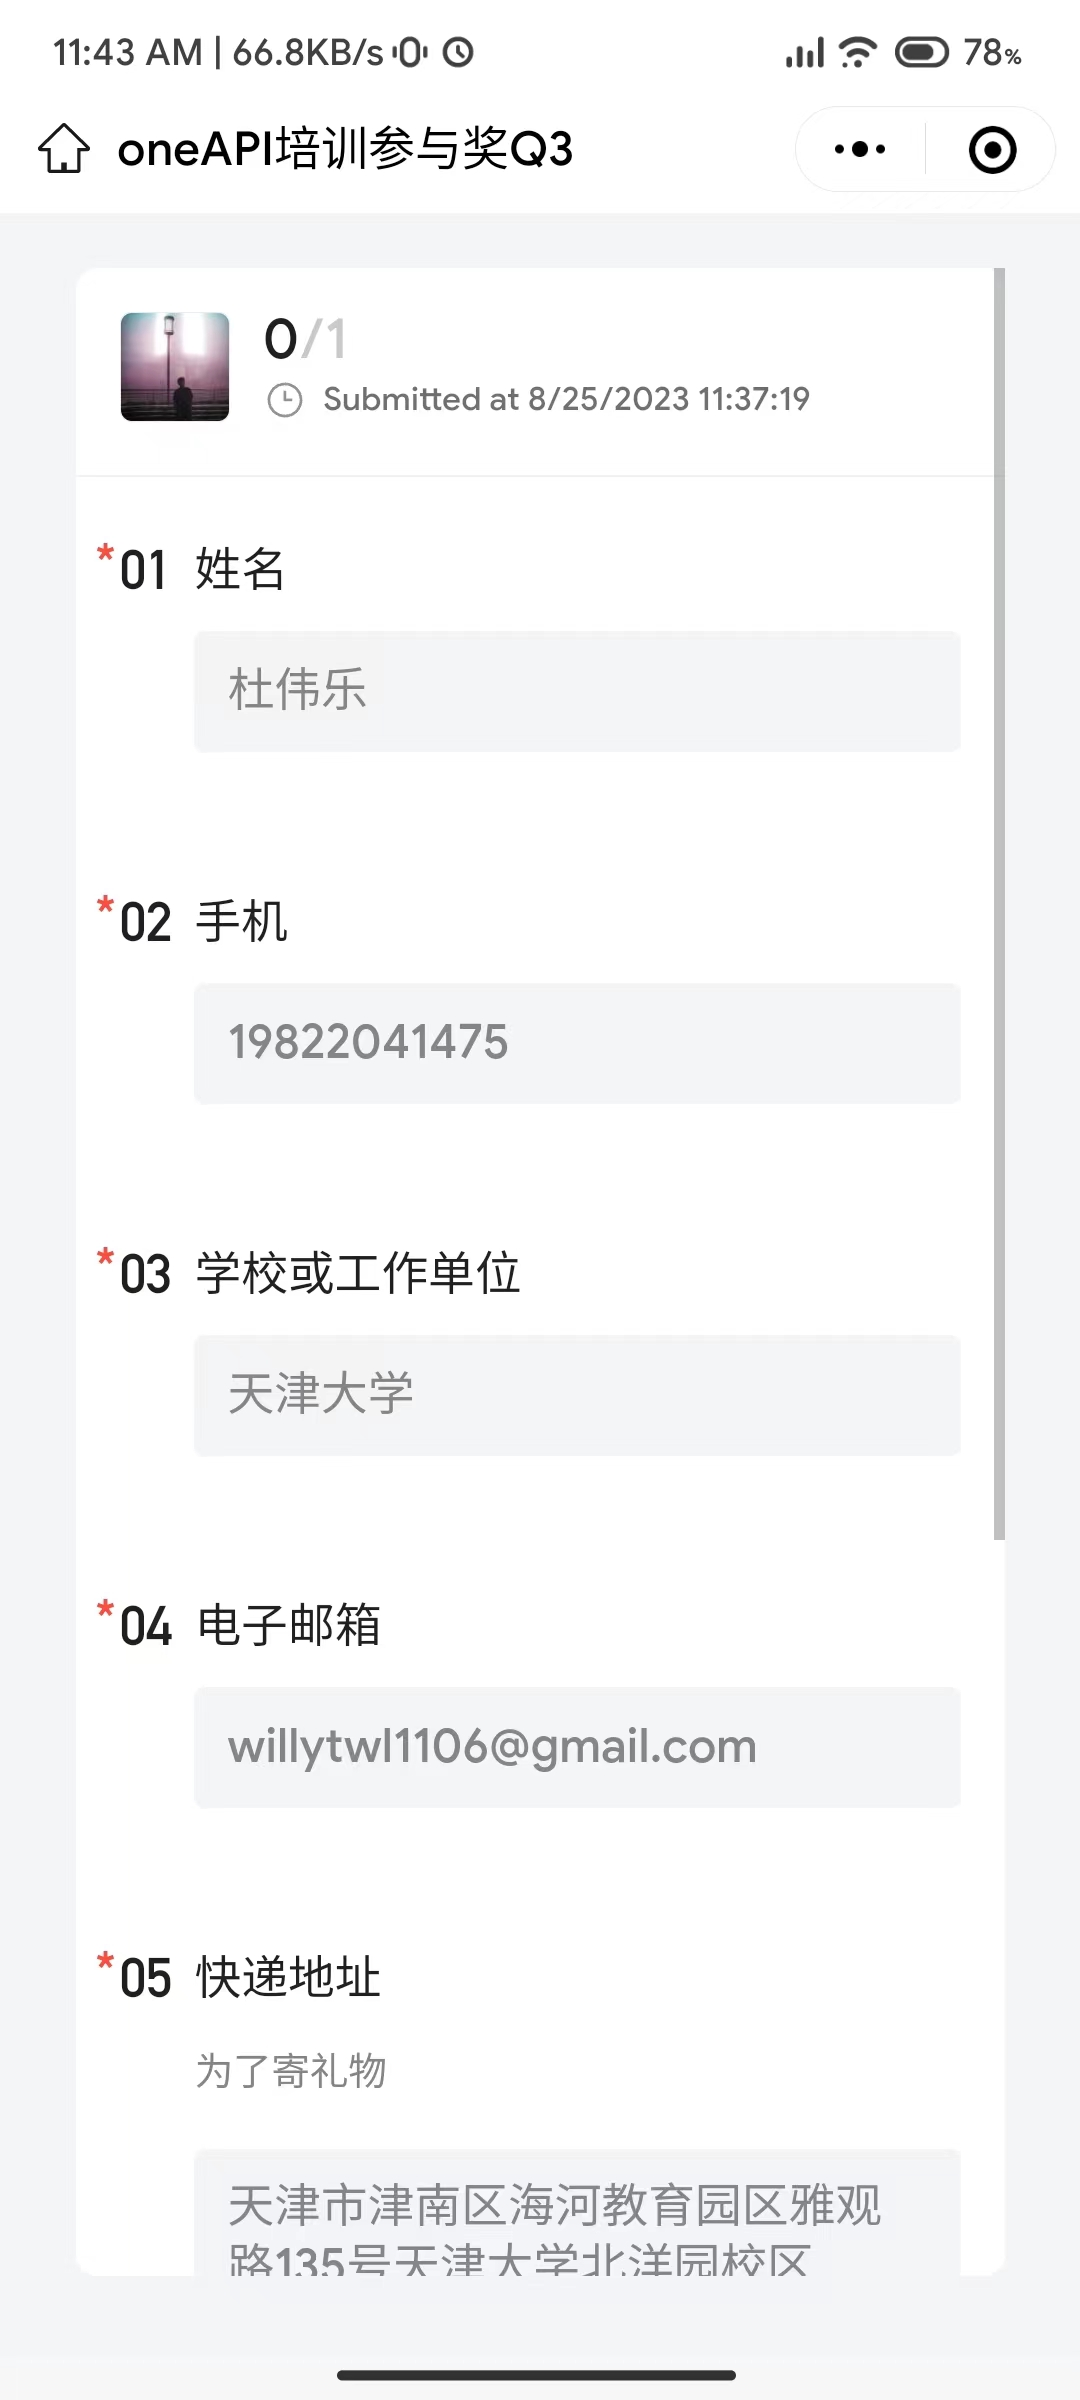
\includegraphics[width=\textwidth]{6321012105_form}
        \caption{6321012105 杜伟乐}\label{fig:6321012105_form}
    \end{minipage}
\end{figure}
 %附件

	% \clearpage

\end{CJK*}                                     % 结束中文字体使用
\end{document}                                 % 结束全文
